\chapter{Hardware Details}\label{app:hard_appendix}

\section{Additional technical information on Game Towers}

\begin{figure}[h]
    \centering
    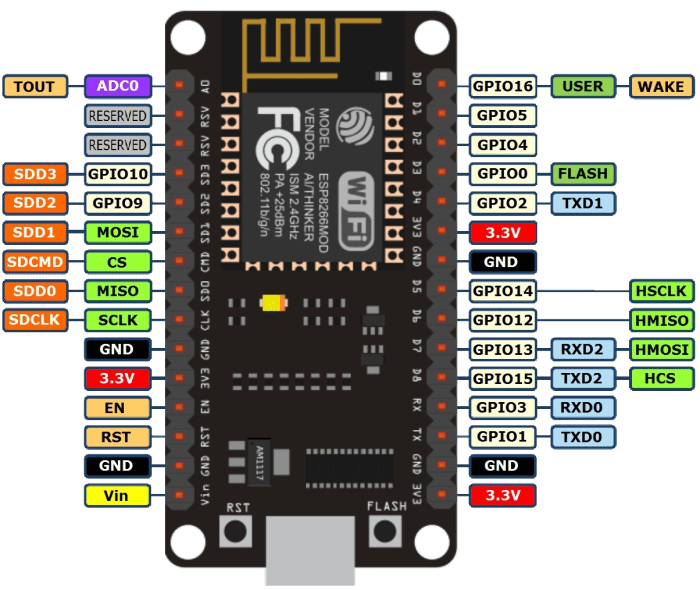
\includegraphics[width=5cm]{images/03-foundation/node_mcu_pinout}
  \caption{The pinout of the NodeMCU V3 ESP8266 ESP-12E WiFi module used for data transmission.}
  \label{fig:tower_board}
\end{figure}

\begin{figure}[H]
	\centering
	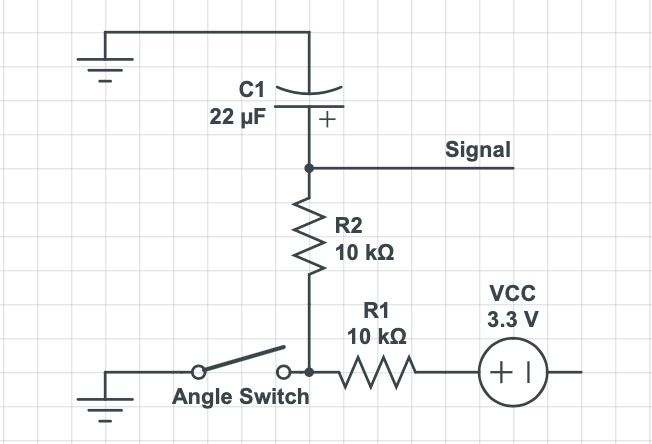
\includegraphics[width=5cm]{images/03-foundation/tilt_sensor_circuit}
	\caption{The circuit for detecting when a tower has fallen. A tilt switch detects the inclination and the low-pass filter smooths out noise from vibrations such as those caused by the player touching the tower. The signal wire is attached to a pin on the NodeMCU V3 ESP8266 ESP-12E WiFi Module, which allows communication with the robot's onboard computer.}
    \label{fig:tilt_circuit} 
\end{figure}

As power supply for the towers, a 7.4V LiPo battery was used on each tower as can been seen on figure~\ref{fig:tower_electronics}. The nominal voltage for the boards was 5V, which is supplied through a voltage regulator.

\begin{lstlisting}[language=C++, label={alg:tower_msg}, caption={Class definition for a message communicating tower led configurations.}]
std_msgs/Header header

uint8 id
bool[3] charge_leds
bool[2] status_led_color

int32 feedback_led_threshold
\end{lstlisting}


\begin{lstlisting}[language=C++, label={alg:buttonTilt_state_msg}, caption={Class definition for a message communicating tower button state and tilt state.}]
std_msgs/Header header
uint8 id
bool value
\end{lstlisting}

The towers maintain a constant communication with the robot via the \verb|game_manage|~\gls{ros} package. The listing~\ref{alg:buttonTilt_state_msg} presents the class definition for messages sent by the towers in response to two main events: a button press (whether of not the button is being currently pressed) and a tilt status (whether the tower has fallen). The same custom message class is used for the two events, but with different~\gls{ros} topic names, making them correspond to their respective sensory inputs independently.

The transmission of button and tilt events makes the \verb|game_manage| update the status of the towers and the game situation to the robot. The listing~\ref{alg:tower_msg} shows the definition of the custom~\gls{ros} message used for indicating which~\glspl{led} should be turned on. The \verb|status_led_color| is separated from the other three \verb|charge_leds| because it is an RGB~\gls{led} (forth~\gls{led} in the tower) used to indicate the status of the tower to the player: it becomes green when the tower has been captured (the player has turned on all four~\glspl{led} by making the necessary button presses); red to indicate the tower has not being capture yet; and blue to indicate the tower has fallen and the player has lost the match. All the first three~\glspl{led} have the same yellow color. The \verb|id| in both classes is used to indicate which tower the message is sent to or received from.

On our system, we have decided to put the logic for turning leds and indicating statuses of the towers separated, \ie in the \verb|game_manage| \gls{ros} package, in order to facilitate changes in the code when needed without having to re-upload specific code to all towers. Additionally, having a central manager allow us to resume operation when facing hardware problems with towers. As an example, the status of towers can be resumed when a tower turns off because of electrical and/or communication problems. Full access to code in in the project repository at GitHub: \url{https://github.com/ewerlopes/phd_robogame.git}.

\section{Computing}
For computing a Shuttle XPC Slim DH270 was used. The device has a 190 $\times$ 165 $\times$ 43~mm steel case, and weights 1.3~kg.  The armature presents two holes for Kensington Locks and numerous threaded holes (M3) at both sides allowing for an easy placement. The operating system used was~\textit{Ubuntu 16.04.3 LTS (64bit)}. The computer had an Intel Core i7 and a~\gls{ram} DDR4 memory of 16 GB.

\section{Control boards}\label{novacore}
The low-level motors actuation and their interface between the~\gls{ros} system have been realized with the Nova Core modules based on STM32-chip\footnote{\url{http://www.novalabs.io/} accessed on \today.}, which implement ready to use components to fulfill robot prototyping requirements with plug \& play approach.  
The provided modules allow to control different type of motors that can be modeled as a second order system, where the input is the voltage applied to the motor armature and output variable is the motor angular speed. Further details about the deployed boards are presented in figure~\ref{fig:boards}.

\begin{figure}[ht]
\centering
 \begin{subfigure}[b]{0.3\textwidth}
 \centering
     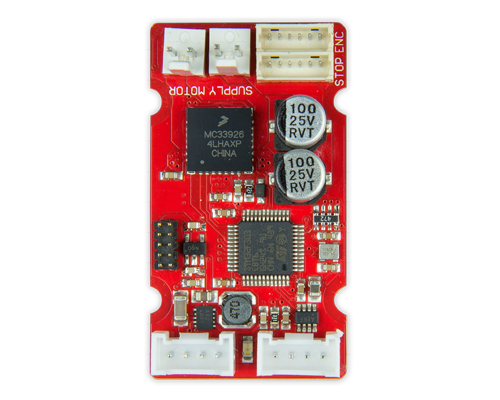
\includegraphics[width=3cm,height=2.5cm]{images/03-foundation/udc}
	\caption{}
 \end{subfigure}
 \begin{subfigure}[b]{0.3\textwidth}
 \centering
     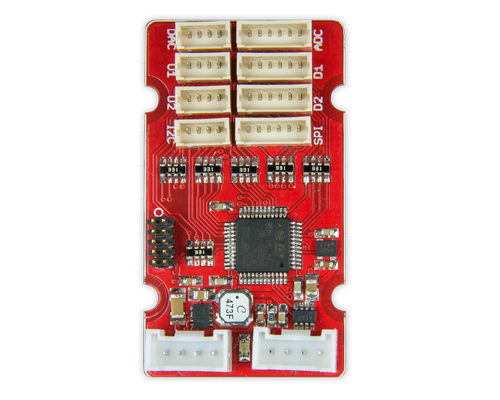
\includegraphics[width=3cm,height=2.5cm]{images/03-foundation/io}
	\caption{}
 \end{subfigure}
 \begin{subfigure}[b]{0.3\textwidth}
 \centering
     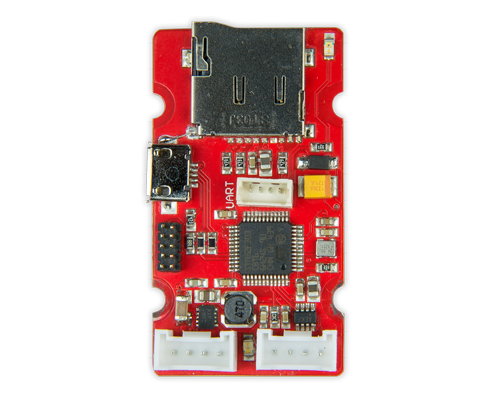
\includegraphics[width=3cm,height=2.5cm]{images/03-foundation/usb}
	\caption{}
	\label{fig:usb_board}
 \end{subfigure}
 \caption{a) UDC board (1 per each motor) capable of driving motors up to 70 W, with torque, speed, and position closed loop control. General attributes: 5-28V supply; 3A max (5A peak); current sense; encoder input; limit switch input; 25 x 45 mm in size. b) IO board (1 per each motor): Integrate existing hardware into the real-time Nova Core bus with analog and digital signals. General attributes: 8 digital GPIO;  4 analog inputs; 2 analog outputs; 2 UART; 1 I2C; 1 SPI; 25 x 45 mm in size. c) USB board (used for data collection) Interface the real-time Nova Core bus with a computer and logs data to microSD memory. General attributes: USB connector;  UART connector; microSD card slot; rosserial support; 25 x 45 mm in size.}
 \label{fig:boards}
\end{figure}

\section{Kinematics of a 3-wheeled omni-directional robot}\label{sec:kinematics}
The pose of a rigid mobile robot is commonly described by six variables, its three-dimensional Cartesian coordinates and its three Euler angles (roll, pitch, yaw) relative to an external coordinate frame~\citep{thrun_probabilistic_2005}. If the robot is considered as moving on a planar surface, this reduces to two Cartesian coordinates and an orientation angle.
The kinematic model of an omni-directional base consists of an equation of motion of the robot in function of wheels velocity without considering the forces acting on the system. In this section, a kinematic model for a 3-wheeled omni-directional robot will be derived.

\begin{figure}[H]
  \centering
  \begin{subfigure}[b]{0.4\textwidth}
     \centering
      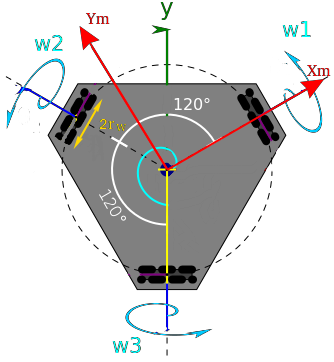
\includegraphics[width=4cm, height=3.5cm]{images/03-foundation/triskarbase1}
	\caption{}
	\label{triskar1} 
  \end{subfigure}
  \begin{subfigure}[b]{0.4\textwidth}
  \centering
      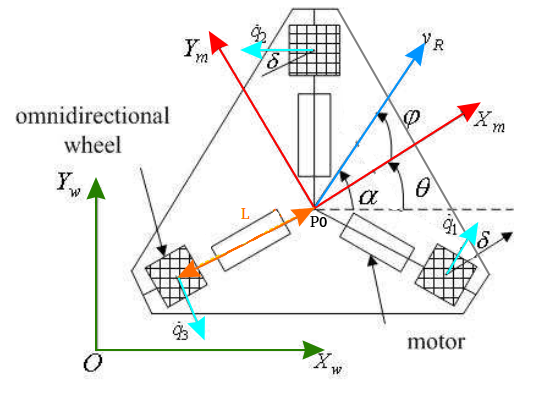
\includegraphics[width=4cm, height=3.5cm]{images/03-foundation/triskarbase2}
	\caption{}
	\label{triskar2} 
  \end{subfigure}
  \caption{Kinematics diagram of the base of an omnidirectional robot. a) omnidirectional base wheels displacement angle. b) the omnidirectional base reference frames and velocities.}
\end{figure}

Considering the figure (\ref{triskar2}), each wheel of the robot is driven by a DC motor and its center has the same distance L to the robot center of mass $P_0$. we define the fixed world coordinate system [$X_R$, $Y_R$] and a mobile robot fixed frame [${x}^m_R$, ${y}^m_R$] that is parallel to the floor and whose origin locates at $P_0$.\\
The robot's orientation is denoted by angle $\theta$, which is the direction angle of the axis $X_m$ in the world coordinate system (positive in the
counterclockwise direction) and $\delta$ refers to the wheel orientation in the robot coordinate system and it is equal to 30 degrees in our considered example.
\\
$\alpha$ and $\phi$ denote the direction of the robot translation velocity $v_R$ observed in the world and robot coordinate systems, respectively.\\
We consider \textbf{v} = [$\dot{x}^m_R,\dot{y}^m_R,\omega$]$^T$ the robot velocities observed in the robot coordinate system; \\
$\mathbf{\dot{q}}$ = [$\dot{q}_1,\dot{q}_2,\dot{q}_3$]$^T$ is the vector of wheel velocities equal to the i-th wheel radius $r_\omega$ multiplied by the wheel angular velocity.

We introduce the transformation matrix from the robot coordinate system to the world coordinate system:
\begin{equation}
^wR_m(\theta)=\begin{bmatrix}
\cos(\theta) &-\sin(\theta)\\
\sin(\theta) & \cos(\theta)\\
\end{bmatrix}
\end{equation}

We can transform from robot to world coordinates system as:
\begin{equation}
\begin{bmatrix}
\dot{x}_R\\
\dot{y}_R\\
\dot{\theta}
\end{bmatrix} =
\begin{bmatrix}
\cos(\theta) &-\sin(\theta) & 0\\
\sin(\theta) & \cos(\theta) & 0\\
0 & 0 & 1
\end{bmatrix}
\begin{bmatrix}
\dot{x}^m_R\\
\dot{y}^m_R\\
\omega
\end{bmatrix}
\label{eq:rotation}
\end{equation}

$P_0$ denotes the position of the center of mass with respect to the world frame as:
\begin{equation}
P_0 = 	\begin{bmatrix}
x_R\\
y_R\\
\end{bmatrix}
\end{equation}

The position $[x_i\quad y_i]^T$ of each wheel can be given with respect to the center of mass of the robot, for i=1,2,3:
\begin{equation}
P_i = 	\begin{bmatrix}
x_{Ri}\\
y_{Ri}\\
\end{bmatrix} = 
^wR_m(\theta)\cdot L
\begin{bmatrix}
1\\
0\\
\end{bmatrix}
\end{equation}

Again, considering that the wheels present a displacement of $120^\circ$ between each other we can deduce the following three vectors:

\begin{equation}
\begin{cases} 
P_1 = 	
^wR_m(0)\cdot L
\begin{bmatrix}
1\\
0\\
\end{bmatrix} =
L
\begin{bmatrix}
1\\
0\\
\end{bmatrix}
\\ 
P_2 = 	
^wR_m(\frac{2\pi}{3})\cdot L
\begin{bmatrix}
1\\
0\\
\end{bmatrix} =
\cfrac{L}{2}
\begin{bmatrix}
-1\\
\sqrt{3}\\
\end{bmatrix}
\\ 
P_3 = 	
^wR_m(\frac{4\pi}{3})\cdot L
\begin{bmatrix}
1\\
0\\
\end{bmatrix} =
-\cfrac{L}{2}
\begin{bmatrix}
-1\\
\sqrt{3}\\
\end{bmatrix}
\\ 
\end{cases} 
\end{equation}

We now define the normal unit vectors of each wheel, representing the translational direction, as follows:
\begin{equation}
D_i =  \frac{1}{L}R(\frac{\pi}{2})P_i\qquad i=1,2,3 \\
\end{equation}
\begin{equation}
\begin{cases}
D_1 = \begin{bmatrix}0 \\ 1 \end{bmatrix} \\
D_2 = -\cfrac{1}{2}\begin{bmatrix}\sqrt{3} \\ 1 \end{bmatrix} \\
D_3 = \cfrac{1}{2}\begin{bmatrix}\sqrt{3} \\ -1 \end{bmatrix} \\
\end{cases}
\end{equation}

Then the translational velocity $q_i$ as depicted in figure~\ref{triskar2} can be written in the robot reference frame as follows:
\begin{equation}
\begin{cases}
\dot{q_1} =\cos(\delta)\dot{x^m _R}+\sin(\delta)\dot{y^m _R}+L{\omega}\\
\dot{q_2} =-\cos(\delta)\dot{x^m _R}+\sin(\delta)\dot{y^m _R}+L{\omega}\\
\dot{q_3} =-\dot{y^m _R}+L{\omega}\\
\end{cases}
\end{equation}

The kinematic model with respect to the robot coordinate system is given by:
\begin{equation}
\begin{bmatrix}
\dot{x}^m _R\\
\dot{y}^m _R\\
{\omega}
\end{bmatrix} =
\begin{bmatrix}
\cos(\delta) & \sin(\delta) & L\\
-\cos(\delta) & \sin(\delta) & L\\
0 & -1 & L
\end{bmatrix}^{-1}
\begin{bmatrix}
\dot{q_1}\\
\dot{q_2}\\
\dot{q_3}\\
\end{bmatrix}	
\label{model1}
\end{equation}
\begin{equation*}
	\begin{bmatrix}
		\dot{x}^m _R\\
		\dot{y}^m _R\\
		{\omega}
	\end{bmatrix} =
	\begin{bmatrix}
		\frac{\sqrt{3}}{3} & -\frac{\sqrt{3}}{3} & 0\\
		\frac{1}{3} & \frac{1}{3} & -\frac{2}{3}\\
		\frac{1}{3L} & \frac{1}{3L} & \frac{1}{3L}
	\end{bmatrix}
	\begin{bmatrix}
		\dot{q_1}\\
		\dot{q_2}\\
		\dot{q_3}\\
	\end{bmatrix}	
\end{equation*}

If we now consider the equation~\ref{eq:rotation} the kinematic model with respect to the world coordinate system is described as:
\begin{equation}
\begin{bmatrix}
\dot{x}_R\\
\dot{y}_R\\
\dot{\theta}
\end{bmatrix} =
\begin{bmatrix}
\frac{2}{3}\cos(\theta+\delta) & -\frac{2}{3}\cos(\theta-\delta) & \frac{2}{3}\sin(\theta)\\
\frac{2}{3}\sin(\theta+\delta) & -\frac{2}{3}\sin(\theta-\delta) & \frac{2}{3}\cos(\theta)\\
\frac{1}{3L} & \frac{1}{3L} & \frac{1}{3L}
\end{bmatrix}
\begin{bmatrix}
\dot{q_1}\\
\dot{q_2}\\
\dot{q_3}\\
\end{bmatrix}	
\label{model2}
\end{equation}

where $\mathbf{\dot{x}}$ = [$\dot{x}_R,\dot{y}_R,\dot{\theta}$]$^T$ is the robot velocity vector with respect to the world coordinate system;

It is important to notice that the transformation matrix in model~\ref{model1} is full rank, which denotes that the translation and rotation of the robot are decoupled, and guarantees the separate control of these two movements.

Low level actuation (such as velocity control of the wheels) is embedded in the robot boards and, after considering figure~\ref{triskar1} and figure~\ref{triskar2}, we can define a system of equations that describes the angular velocity of each wheel. If we define $[\omega_{R_1}; \omega_{R_2}; \omega_{R_3}]^T$ as the wheel angular velocities vector, we have:
\begin{equation}
\begin{cases} 

\omega_{R1} = \dot{x}^m_R\cos(\delta)+\dot{y}^m_R\sin(\delta)+ \omega L\\ 
\omega_{R2} = -\dot{x}^m_R\cos(\delta)+\dot{y}^m_R\sin(\delta)+\omega L\\ 
\omega_{R3} = -\dot{y}^m_R +  \omega L \\ 
\end{cases} 
\end{equation}
This can be written in matrix form as:
\begin{equation}
\begin{bmatrix}
\omega_{R1}\\
\omega_{R2}\\
\omega_{R3}
\end{bmatrix} = 
\begin{bmatrix}
\cos(\delta) & \sin(\delta) & L \\
-\cos(\delta) & \sin(\delta) & L \\
0 & -1 & L
\end{bmatrix}
\begin{bmatrix}
\dot{x}^m_R\\
\dot{y}^m_R\\
\omega
\end{bmatrix}
\end{equation} 
As previously anticipated we can also say:
\begin{equation}
\begin{bmatrix}
\dot{q_1}\\
\dot{q_2}\\
\dot{q_3}\\
\end{bmatrix} = 
r_\omega
\begin{bmatrix}
\omega_{R1}\\
\omega_{R2}\\
\omega_{R3}
\end{bmatrix}
\end{equation}
It is also known that a further relation between motor velocity and wheel velocity exists and is given by the equation:
\begin{equation}
\omega_{Ri}=\frac{r_\omega}{\eta N}\omega_{mi}
\end{equation}
for i=1,2,3 where $r_\omega$ is the wheel radius, N is the coupling factor and $\eta$ is the wheel/motor coupling efficiency factor.

The direct kinematic for an holonomic robot can be finally written as:
\begin{equation}
\begin{bmatrix}
\dot{x}_R\\
\dot{y}_R\\
\dot{\theta}
\end{bmatrix} =
\begin{bmatrix}
\frac{2}{3}\cos(\theta+\delta) & -\frac{2}{3}\cos(\theta-\delta) & \frac{2}{3}\sin(\theta)\\
\frac{2}{3}\sin(\theta+\delta) & -\frac{2}{3}\sin(\theta-\delta) & \frac{2}{3}\cos(\theta)\\
\frac{1}{3L} & \frac{1}{3L} & \frac{1}{3L}
\end{bmatrix}
\frac{r_\omega}{\eta N}
\begin{bmatrix}
\omega_{m1}\\
\omega_{m2}\\
\omega_{m3}
\end{bmatrix}
\label{directkin}
\end{equation}
\paragraph{Inverse Kinematic:} If we reverse and re-arrange equation~\ref{directkin} we obtain:
\begin{equation}
B = \begin{bmatrix}
\frac{2}{3}\cos(\theta+\delta) & -\frac{2}{3}\cos(\theta-\delta) & \frac{2}{3}\sin(\theta)\\
\frac{2}{3}\sin(\theta+\delta) & -\frac{2}{3}\sin(\theta-\delta) & \frac{2}{3}\cos(\theta)\\
\frac{1}{3L} & \frac{1}{3L} & \frac{1}{3L}
\end{bmatrix}
\end{equation}
\begin{equation}
\begin{bmatrix}
\dot{x}_R\\
\dot{y}_R\\
\dot{\theta}
\end{bmatrix} =
B
\frac{r_\omega}{\eta N}
\begin{bmatrix}
\omega_{m1}\\
\omega_{m2}\\
\omega_{m3}
\end{bmatrix}
\end{equation}
\begin{equation}
\begin{bmatrix}
\omega_{m1}\\
\omega_{m2}\\
\omega_{m3}
\end{bmatrix}=
\frac{\eta N}{r_\omega}B^{-1}
\begin{bmatrix}
\dot{x}_R\\
\dot{y}_R\\
\dot{\theta}
\end{bmatrix}
\label{inversekin}
\end{equation}
Equation~\ref{inversekin} represents the inverse kinematic model for the considered holonomic robot that bounds the robot velocities in the inertial reference frame to the actual motors velocities.

\section{Microsoft Kinect\textsuperscript{\textregistered} One specifications}
\begin{figure}[H]
	\centering
	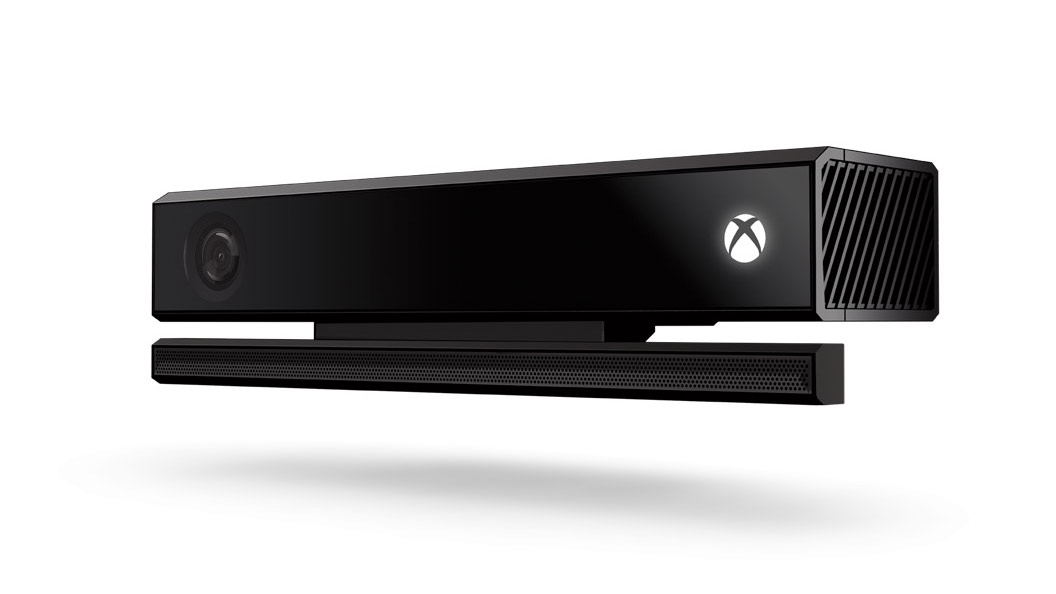
\includegraphics[width=5cm]{images/03-foundation/kinect}
	\caption{Microsoft Kinect\textsuperscript{\textregistered} for Xbox ONE.}
	\label{kinect} 
\end{figure}

\begin{table}[H]
\begin{center}
	\begin{tabular}{|c|c|}
		\hline
		sensor dimensions & 24.9 cm $\times$ 6.6 cm $\times$ 6.7 cm\\
		\hline
		sensor weight & approximately 3.1 lbs (1.4 kg) \\
		\hline
		sensor FOV & 70\textsuperscript{$\circ$} x 60\textsuperscript{$\circ$} \\
		\hline
		depth sensing resolution & 512 x 424 \\
		\hline
		max - min depth & 4.5m - 0.4m \\ 
		\hline
		working frequency & 30 hz \\
		\hline 
	\end{tabular}
\end{center}
\caption{Microsof Kinect\textsuperscript{\textregistered} sensor features.}
\label{kinectfeatures}
\end{table}

\subsection{Motors}
The three motors are MAXON 118798 DC motor RE36 GB 70W KL 2WE, whose characteristics are reported in Figure~\ref{motor} and Table~\ref{maxon}.

\begin{figure}[h]
	\centering
	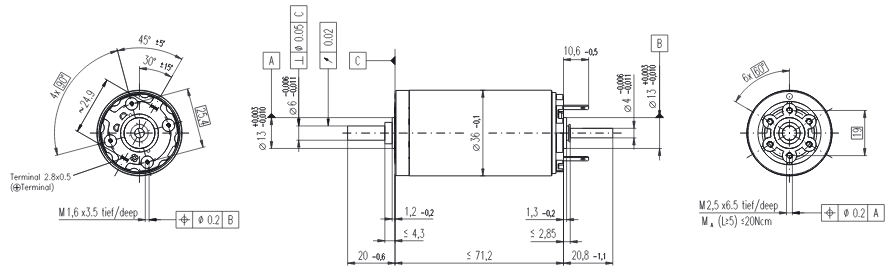
\includegraphics[width=\textwidth]{images/03-foundation/motor}
	\caption{MAXON 118798 DC motor schematic. Three units were used in our platform.}
	\label{motor} 
\end{figure}

\begin{table}[h]
	\begin{center}
		\begin{tabular}{|c|c|}
			\hline
			Assigned power rating &  70 W \\
			\hline
			Nominal voltage & 24 V \\
			\hline
			No load speed & 70 x 60  \\
			\hline
			Stall torque & 783 mNm \\
			\hline
			No load current & 105 mA \\ 
			\hline
			Terminal resistance & 1.11 ohm \\
			\hline 
			Max. permissible speed & 8200 rpm \\
			\hline
			Max. efficiency &  85\% \\
			\hline
			Torque constant & 36.4 mNm/A \\
			\hline
			Speed constant & 263 rpm/V \\
			\hline
			Mechanical time constant & 6 ms \\
			\hline 
			Rotor inertia & 67.7 gcm$^2$ \\
			\hline
			Terminal Inductance & 0.2 mH \\
			\hline  
			reduction ratio & [14 : 1] (166158 planetary gear GP32A 2.25NM) \\
			\hline 
		\end{tabular}
	\end{center}
	\caption{MAXON 118798 DC motor parameters.}
    \label{maxon}
\end{table}

\subsubsection{Encoders}
On each motor a 110513 tacho ENCODER HEDS 5540 500IMP 3K is mounted to get the speed of the motor, whose characteristics are reported in Figure~\ref{enc}.

\begin{figure}[h]
	\centering
	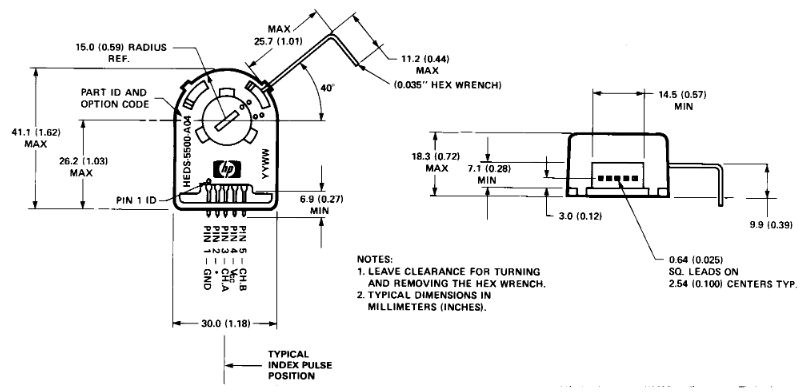
\includegraphics[width=\textwidth]{images/03-foundation/enc}
	\caption{Motor encoders deployed for motion sensing and control.}
	\label{enc} 
\end{figure}

Encoders contain a single Light Emitting Diode (LED) as its light source. The light is collimated into a parallel beam by means of a single lens located directly over the LED. Opposite the emitter is the integrated detector circuit. This IC consists of multiple sets of photodetectors and the signal processing circuitry necessary to produce the digital waveforms. The code-wheel rotates between the emitter and detector, causing the light beam to be interrupted by the pattern of spaces and bars on the code-wheel. The photodiodes detect these interruptions and send signals to the signal processing circuitry that produces the final outputs that is an index pulse $P_O$ which is generated once for each full rotation of the code-wheel.

\section{Power distribution}
We have used a rapid discharging lead-acid battery FIAMM 12FGHL34 12V 9Ah. This battery has been designed for optimal performance and protection against power disturbances. Ideal for~\gls{ups} intensive discharge applications, emergency power systems, security systems, data processing centers. Technical characteristics in table~\ref{tab:power_techicals}.

\begin{table}[h]
	\begin{center}
		\begin{tabular}{|c|c|}
		\hline
        Voltage & 12V \\
        \hline 
        Capacity & 20h 9Ah \\
        \hline 
        Size & 15,00 x 7,00 x 10,00 cm \\
        \hline 
        Weight & 2,90 Kg \\
        \hline 
        Connectors & Faston 6,3 \\
        \hline 
        Application & Alarm systems, Emergency lights, Renewable energies, \gls{ups}.\\
        \hline 
    \end{tabular}
    \caption{Technical characteristics of the FIAMM 12FGHL34 lead-acid battery.}
    \label{tab:power_techicals}
    \end{center}
\end{table}

\section{Additional tower navigation details}
Recall that the equation~\ref{eq:rotation} allows us to perform the transformation from reference frames. The $x$ and $y$ robot position in robot frame is defined as $\dot{\bar{x}}_R^m$ and $\dot{\bar{y}}_R^m$, respectively. Another problem that must be considered at this point is to guarantee the decoupling between robot rotations and translations (the control of the robot orientation must be completely independent from the xy-translation, since this will enable the robot to track the movement of the human player while navigating during the game). 

Let us consider again the equation~\ref{model2} introduced in section~\ref{sec:kinematics}
\begin{equation*}
	\begin{bmatrix}
		\dot{x}_R\\
		\dot{y}_R\\
		\dot{\theta}
	\end{bmatrix} =
	\begin{bmatrix}
		\frac{2}{3}\cos(\theta+\delta) & -\frac{2}{3}\cos(\theta-\delta) & \frac{2}{3}\sin(\theta)\\
		\frac{2}{3}\sin(\theta+\delta) & -\frac{2}{3}\sin(\theta-\delta) & \frac{2}{3}\cos(\theta)\\
		\frac{1}{3L} & \frac{1}{3L} & \frac{1}{3L}
	\end{bmatrix}
	\begin{bmatrix}
		\dot{q_1}\\
		\dot{q_2}\\
		\dot{q_3}\\
	\end{bmatrix}	
\end{equation*}
As we already anticipated, the transformation matrix is full rank. A matrix is said to have full rank if its rank equals the largest possible for a matrix of the same dimensions. Now considering the matrix properties, we know that if $A$ is a square matrix ($m = n$), then $A$ is invertible if and only if $A$ has rank $n$ (that is, $A$ has full rank).\\
For the high-level control laws without considering the wheel velocities, the kinematic model is given as:
\begin{equation}
\begin{bmatrix}
\dot{\bar{x}}_R\\
\dot{\bar{y}}_R\\
\dot{\bar{\theta}}_R
\end{bmatrix}
= G
\begin{bmatrix}
\dot{\bar{x}}_R^m\\
\dot{\bar{x}}_R^m\\
\dot{\omega}
\end{bmatrix}
\label{eq:control_law}
\end{equation}
where:

\begin{equation}
G=\begin{bmatrix}
^wR_m(\theta) & 0\\
0 & 1\\
\end{bmatrix}\qquad
^wR_m(\theta)=\begin{bmatrix}
\cos(\theta) &-\sin(\theta)\\
\sin(\theta) & \cos(\theta)\\
\end{bmatrix}
\end{equation}

As already stated in section~\ref{sec:kinematics}, $^wR_m(\theta)$ is the transformation matrix from the robot coordinate system to the world coordinate system. Since G is full rank, the characteristics of decoupled movements are also kept in equation~\ref{eq:control_law}.

As anticipated, it is now necessary to transform the velocities from world frame to robot body frame, the trigonometric functions of angle $\theta$ in the transformation matrix $G$ determine the non-linearities of the model. Since the matrix G is full rank, this nonlinear model can be exactly linearized by introducing a simple compensator~\citep{li_motion_2009}.

We define an \textit{Inverse Input-Output Linearization} based control approach where:

\begin{equation}
    C = G^{-1},
\end{equation} 

denotes that the translation and rotation of the robot are decoupled, and guarantees the separate control of these two movements. The linearized system becomes $\mathbf{\dot{x}} = \mathbf{u}$ with a new input vector \textbf{u} = [$u_1,u_2,u_3$]$^T$.

\begin{figure}[H]
	\centering
	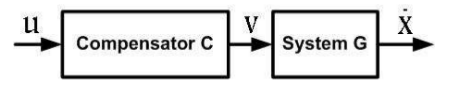
\includegraphics[width=10cm]{images/03-foundation/comp1}
	\caption{Linearized system by the component C.} 
	\label{comp1}
\end{figure}

Figure~\ref{comp1} shows a linear system completely decoupled and enable to control the robot translation and rotation in a separate way. \\
When a controller $K$ is designed based on this simple linear system, the controller of the original system is generated as $CK$. The overall control loop, consists of the nonlinear system, the compensator, and the controller shown below:

\begin{figure}[H]
	\centering
	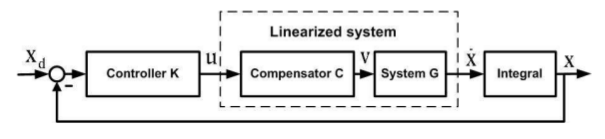
\includegraphics[width=12cm]{images/03-foundation/comp2}
	\caption{Closed-loop control system.} 
	\label{comp2}
\end{figure}

Considering figure~\ref{comp2}, $\mathbf{x_d}$ is a vector of desired positions to reach, or way-points.
Based on this input-output linearized system, path following and orientation tracking problems can be analyzed with respect to the robot translation and rotation control.

The outputs of algorithm~\ref{alg:pointopoint} will then be the input of the compensator shown in figure~\ref{comp1}, and its outputs will be $\dot{\bar{x}}_R^m$ and $\dot{\bar{y}}_R^m$, which are the required velocity set points of the robot considering the robot reference frame.

\begin{algorithm}[h]
	\# Transform the un-smoothed velocity set-points [$\dot{\bar{x}}_R$, $\dot{\bar{y}}_R$] from world frame to robot reference frame, while keeping linear and angular movements of the robot decoupled.\;
	$G=\begin{bmatrix}
	^wR_m(\theta) & 0\\
	0 & 1\\
	\end{bmatrix}$\;
	\# Define C matrix and world-frame velocity vector\;
	$C = G^{-1}$\;
	$\dot{x}=[\dot{\bar{x}}_R, \dot{\bar{y}}_R]$\;
	\# Convert velocity commands from world to robot frame\;
	$\begin{bmatrix}
	\dot{\bar{x}}_R^m\\
	\dot{\bar{y}}_R^m\\
	\end{bmatrix}=C
	\begin{bmatrix}
	\dot{\bar{x}}_R\\
	\dot{\bar{y}}_R\\
	\end{bmatrix}
	$\;
	\Return $\dot{\bar{x}}_R^m$, $\dot{\bar{y}}_R^m$
	\caption{Linear compensation and world-to-body transformation of the velocity set-point} 
	\label{alg:compensator}
\end{algorithm}

With this approach, the velocity set-points $\dot{\bar{x}}_R^m$ and $\dot{\bar{y}}_R^m$, returned from the algorithm~\ref{alg:compensator}, dynamically change during the game and often the variation has a step-function shaped form that causes the low level actuation to react violently to make the robot reaching the desired velocity, especially when starting from the initial position with 0-velocity (see figures~\ref{vel14} and~\ref{wheel14}).
This will result in the robot wheels undergoing in slippage due to the too sharp acceleration required to reach the velocity set-point. This is an undesired effect that is source of non-systematic odometry errors that may lead to instability and loss of localization. A number of tests have been performed to quantify the effect of the wheel slippage during the initial robot acceleration phase. In these tests the robot linearly translates along $x$ and $y$ axis and receives the initial velocity set-point at $1m/s$ or $1.4m/s$. In figures~\ref{opti14},~\ref{amcl14},~\ref{poserror14},~\ref{opti14y},~\ref{amcl14y}, and~\ref{poserror14y} we can see the localization error introduced during the xy-translation.

To avoid this effect, a velocity smoother has been introduced in order to obtain a smooth velocity set-point control signal to be sent to the robot low level actuation to avoid wheels slippage during the  acceleration phase. The inputs of the velocity smoother are the un-smoothed velocity set-points [$\dot{\bar{x}}_R^m$, $\dot{\bar{y}}_R^m$], some of the internal parameters such as maximum allowed velocity and maximum allowed acceleration can be changed online to modify the final response of the robot, t. The output are the final xy-velocity control signals [$\dot{x}_R^m$, $\dot{y}_R^m$] in robot reference frame that will be sent to the low level actuation.

\begin{algorithm}[h]
	\# define initial velocity\;
	$\dot{x}_{(t-1)}$ = $\left[{\dot{\bar{x}}_R^m}_{(t-1)},\quad {\dot{\bar{y}}_R^m}_{(t-1)}\right]$\;
	\# Define accelerations\;
	$\ddot{x}= \left[ {\dot{\bar{x}}_R^m}_{(t)}-{\dot{\bar{x}}_R^m}_{(t-1)},\quad {\dot{\bar{y}}_R^m}_{(t)}-{\dot{\bar{y}}_R^m}_{(t-1)}\right]$\;
	\# Acceleration clamping \;
	\eIf{$\ddot{x}\geq\ddot{x}_{\text{max}}$}{
		$\ddot{x}=\ddot{x}_{\text{max}}$\;
	}{
	\If{$\ddot{x}<\ddot{x}_{\text{max}}$}{
		$\ddot{x}=-\ddot{x}_{\text{max}}$\;
	}}
	\# Generate smoothing factor, $K_s$ is a proportional gain, $\dot{\bar{x}}$ is the maximum desired velocity and $T_\text{max}$ is the maximum time elapsed to reach the set-point, all those factors can be tuned ($K_s\cdot T_\text{max} > 0 $)\;
	$\tau = \left| \cfrac{1}{K_s\cdot\cfrac{T_\text{max}}{\dot{x}_{\text{max}}}}\right|\qquad(0\leq\tau\leq1)$\;
	\# Smooth the velocity control signal\;
	${\dot{x}_R^m} = {\dot{\bar{x}}_R^m}_{(t-1)}+\tau\cdot{\dot{\bar{x}}_R^m}_{(t)}-\tau\cdot{\dot{\bar{x}}_R^m}_{(t-1)}$ \;
	${\dot{y}_R^m} = {\dot{\bar{y}}_R^m}_{(t-1)}+\tau\cdot{\dot{\bar{y}}_R^m}_{(t)}-\tau\cdot{\dot{\bar{y}}_R^m}_{(t-1)}$ \;
	\Return $\dot{x}_R^m$, $\dot{y}_R^m$
	\caption{Velocity Smoother} 
	\label{smoother}
\end{algorithm}

With the values reported in table~\ref{parsmoother}, the behavior shown in figure~\ref{controlsweep} has been obtained. The velocity smoother runs together with the Point-to-Point Navigation algorithm to apply robot's velocity and acceleration limits to the incoming commands before re-sending them to the robot. It basically pre-filters any incoming command input based on some acceleration constraints. 

\begin{table}[h]
	\begin{center}
		\begin{tabular}{|c|c|}
			\hline
			Parameter & value\\
			\hline
			$\ddot{x}_{\text{max}}$  & $0.5m/s^2$\\
			\hline
			$\dot{x}_{\text{max}}$  & $0.7m/s$\\
			\hline
			$T_{\text{max}}$  & $3$ sec\\
			\hline
			$K_s$  & $50$ sec\\
			\hline
		\end{tabular}
	\end{center}
	\caption{Velocity Smoother parameters tuning}
	\label{parsmoother}
\end{table}

\begin{figure}[h]
	\centering
	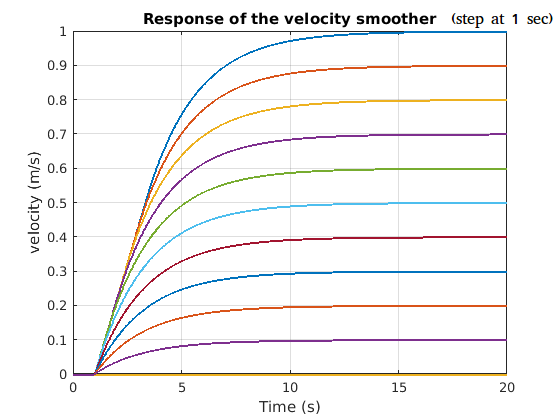
\includegraphics[width=0.8\columnwidth]{images/03-foundation/controlsweep}
	\caption{Smoothing of a step-shaped unsmoothed velocity set-point, at $t=1\text{sec}$ a sweep of 10 step transition set-points is fed as input of the velocity smoother, in the image are shown the smoothed values for each test case} 
	\label{controlsweep}
\end{figure}

\begin{figure}[h]
	\centering
	\begin{subfigure}{6cm}
	    \centering
		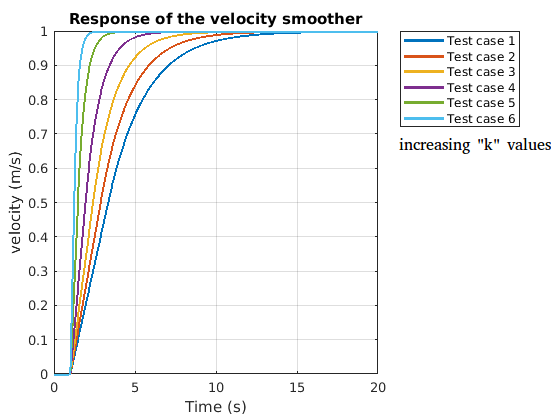
\includegraphics[width=0.95\columnwidth]{images/03-foundation/ksweep}
		\caption{$K_s$ parameter sweep}
		\label{sit1} 
	\end{subfigure}
	~
	\begin{subfigure}{6cm}
	    \centering
		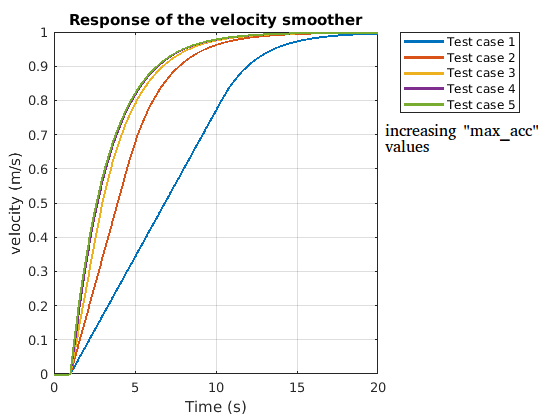
\includegraphics[width=0.95\columnwidth]{images/03-foundation/maxaccsweep}
		\caption{$\ddot{x}_{\text{max}}$ sweep}
		\label{sit2}
	\end{subfigure}
	~
	\begin{subfigure}{6cm}
	    \centering
		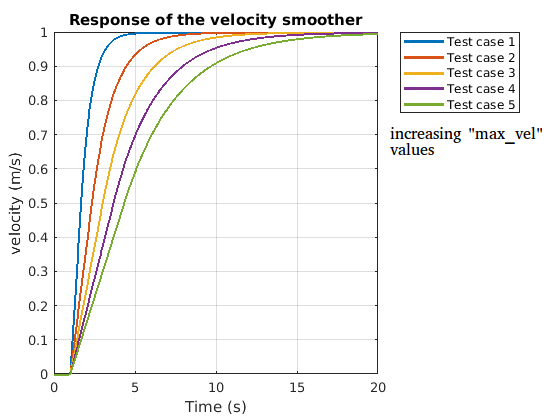
\includegraphics[width=0.95\columnwidth]{images/03-foundation/maxvel}
		\caption{$\dot{x}_{\text{max}}$ parameter sweep}
		\label{sit3} 
	\end{subfigure}
	~
	\begin{subfigure}{6cm}
	    \centering
		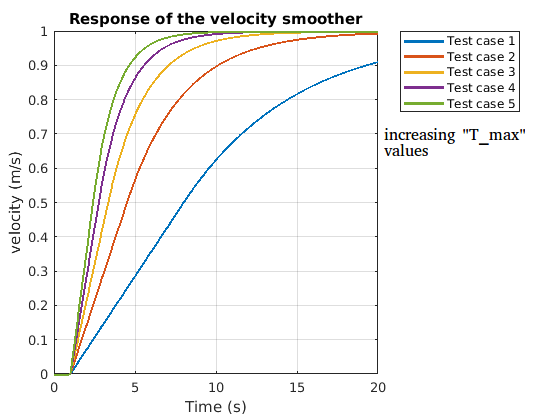
\includegraphics[width=0.95\columnwidth]{images/03-foundation/Tmaxsweep}
		\caption{$T_{\text{max}}$ sweep}
		\label{sit4}
	\end{subfigure}
	\label{param1}
	\caption{Effect of the variation of the various parameters on the final response. In these trials, while varying a parameter, the others were kept at the values shown in table~\ref{parsmoother}}
\end{figure}

\begin{figure}[h]
	\centering
	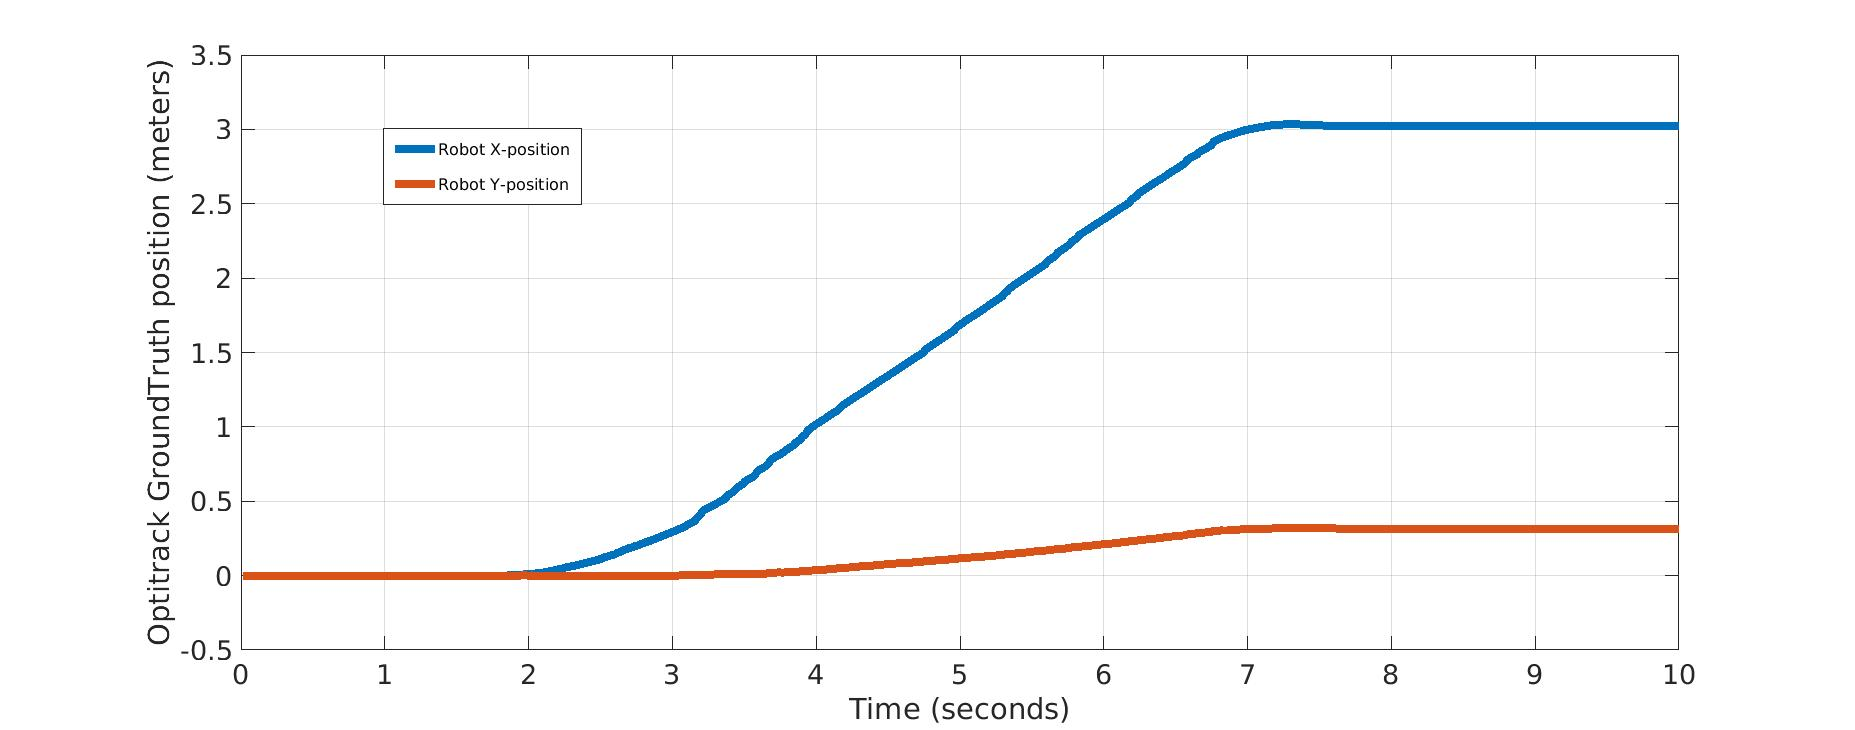
\includegraphics[width=\textwidth]{images/03-foundation/opti14}
	\caption{Ground truth Robot Position - 1.4m/s x-velocity set-point (slipping~/~no velocity smoothing).} 
	\label{opti14}
\end{figure}

\begin{figure}[H]
	\centering
	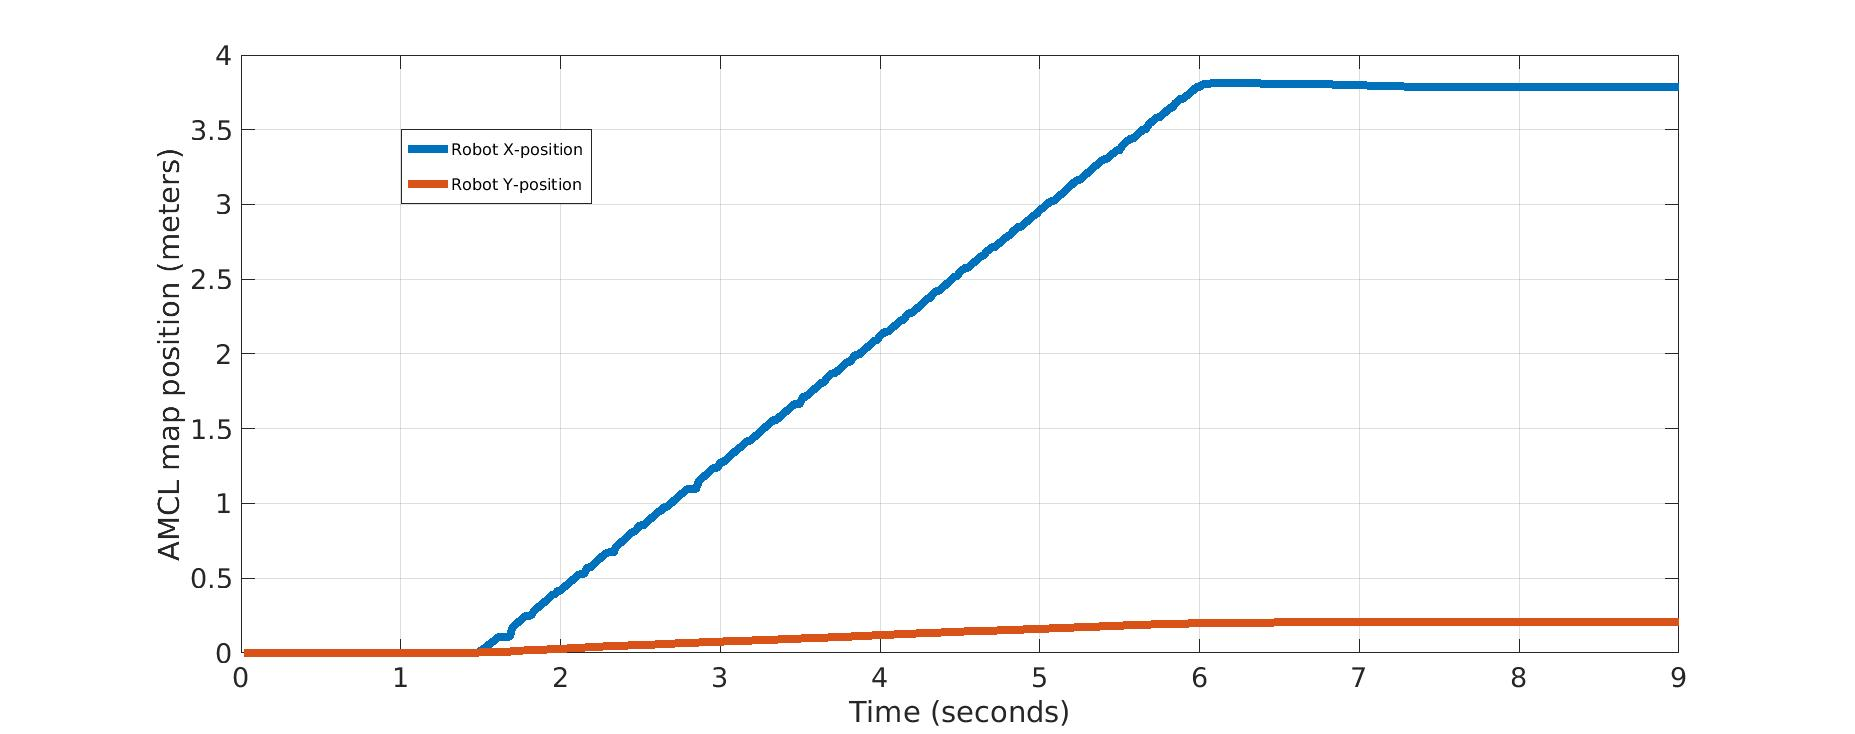
\includegraphics[width=12cm]{images/03-foundation/amcl14}
	\caption{AMCL map position - 1.4m/s x-velocity set-point (slipping / no velocity smoothing).} 
	\label{amcl14}
\end{figure}

\begin{figure}[H]
	\centering
	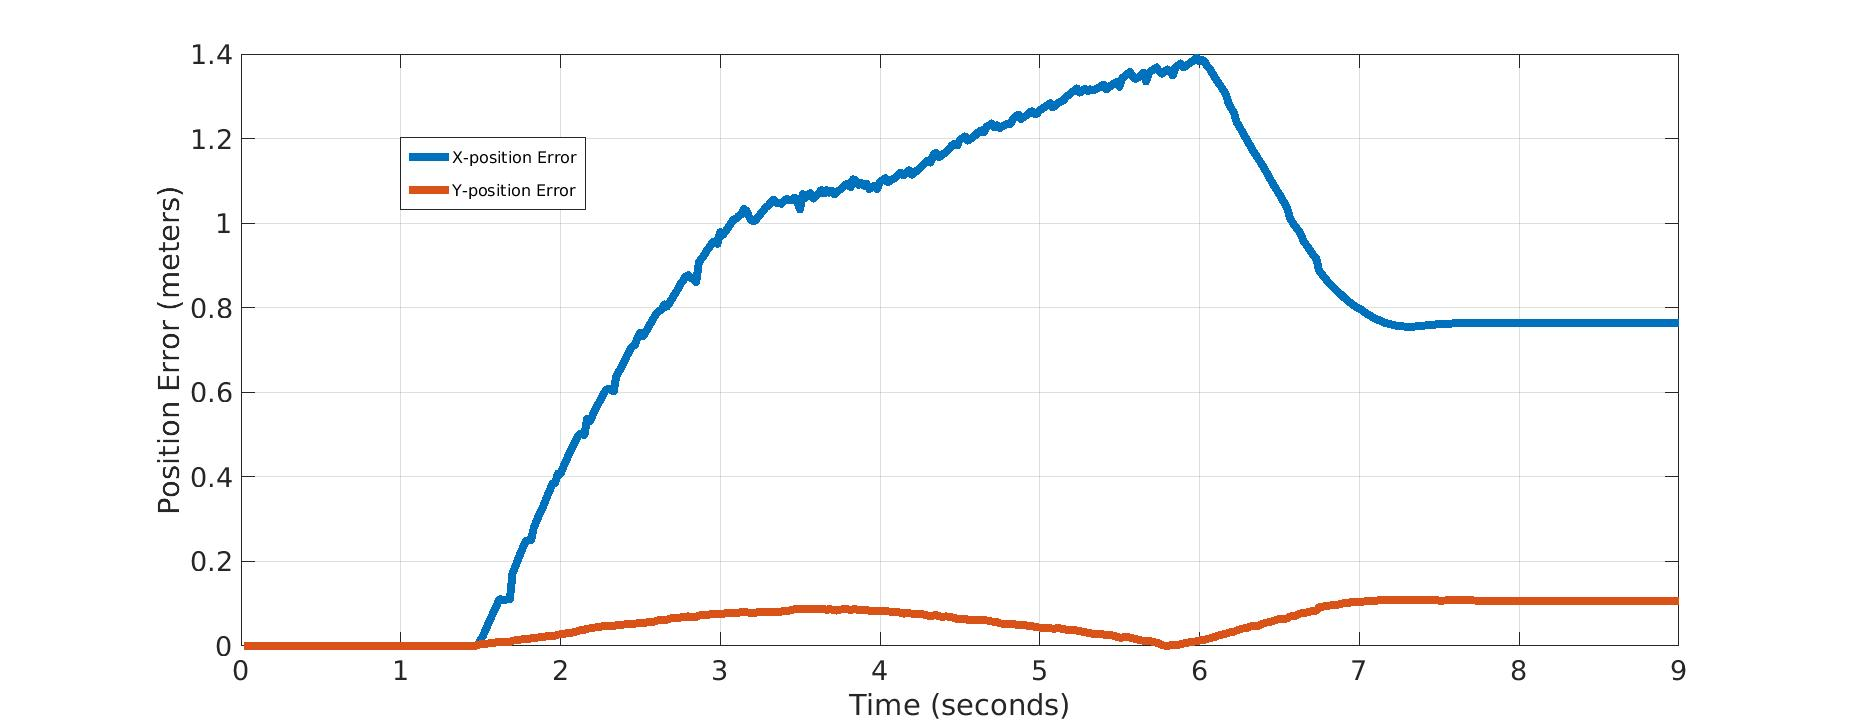
\includegraphics[width=12cm]{images/03-foundation/poserror14}
	\caption{Position error - 1.4m/s x-velocity set-point (slipping / no velocity smoothing).} 
	\label{poserror14}
\end{figure}

\begin{figure}[H]
	\centering
	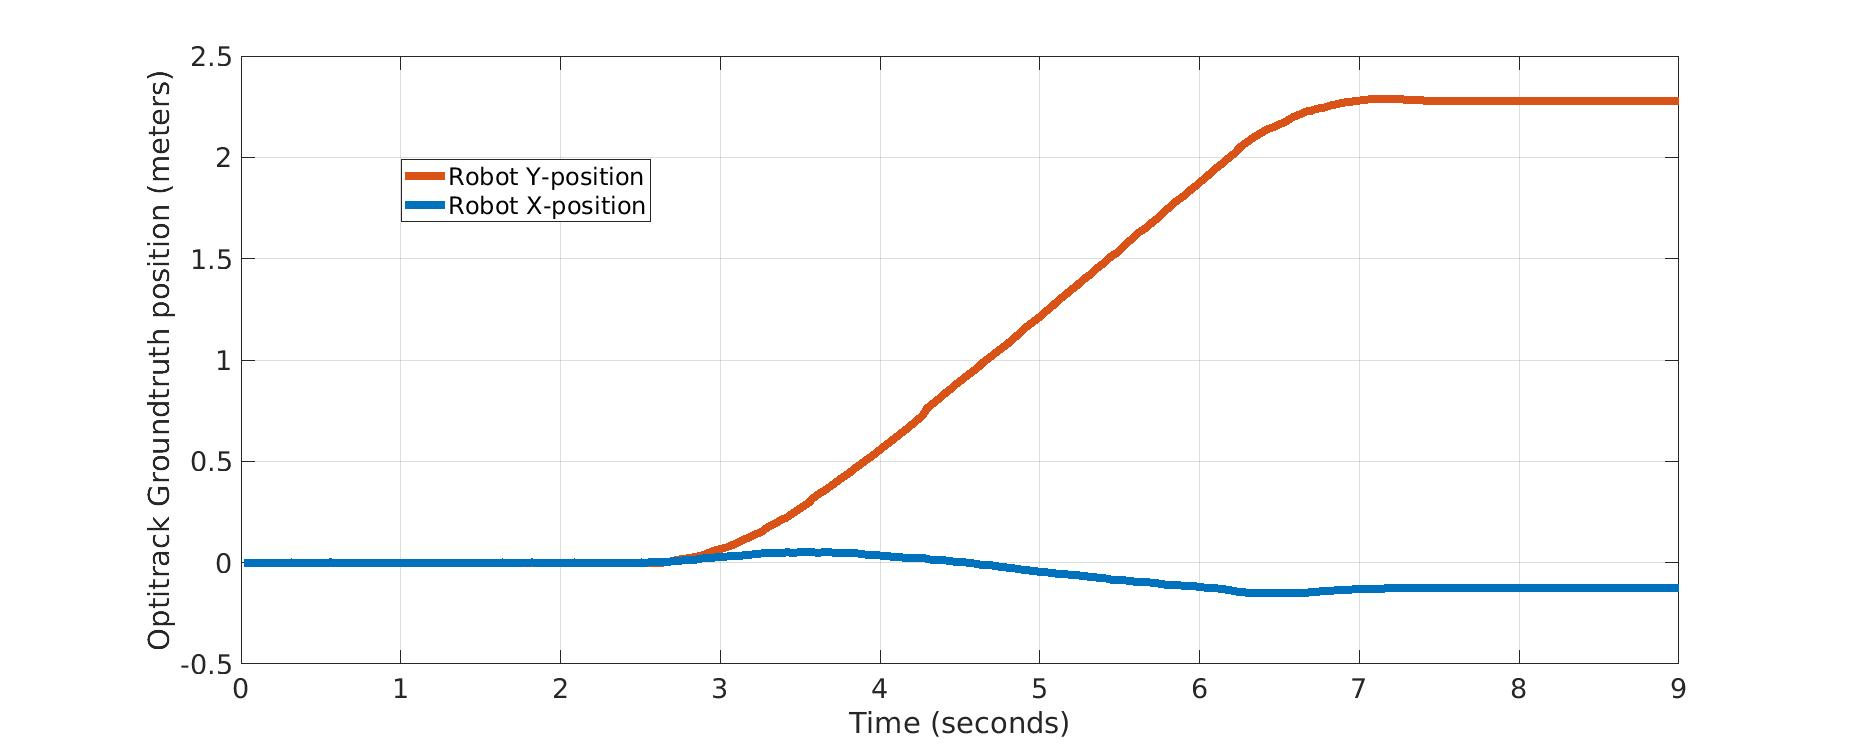
\includegraphics[width=12cm]{images/03-foundation/opti14y}
	\caption{Ground truth Robot Position - 1.4m/s y-velocity set-point (slipping / no velocity smoothing).} 
	\label{opti14y}
\end{figure}

\begin{figure}[H]
	\centering
	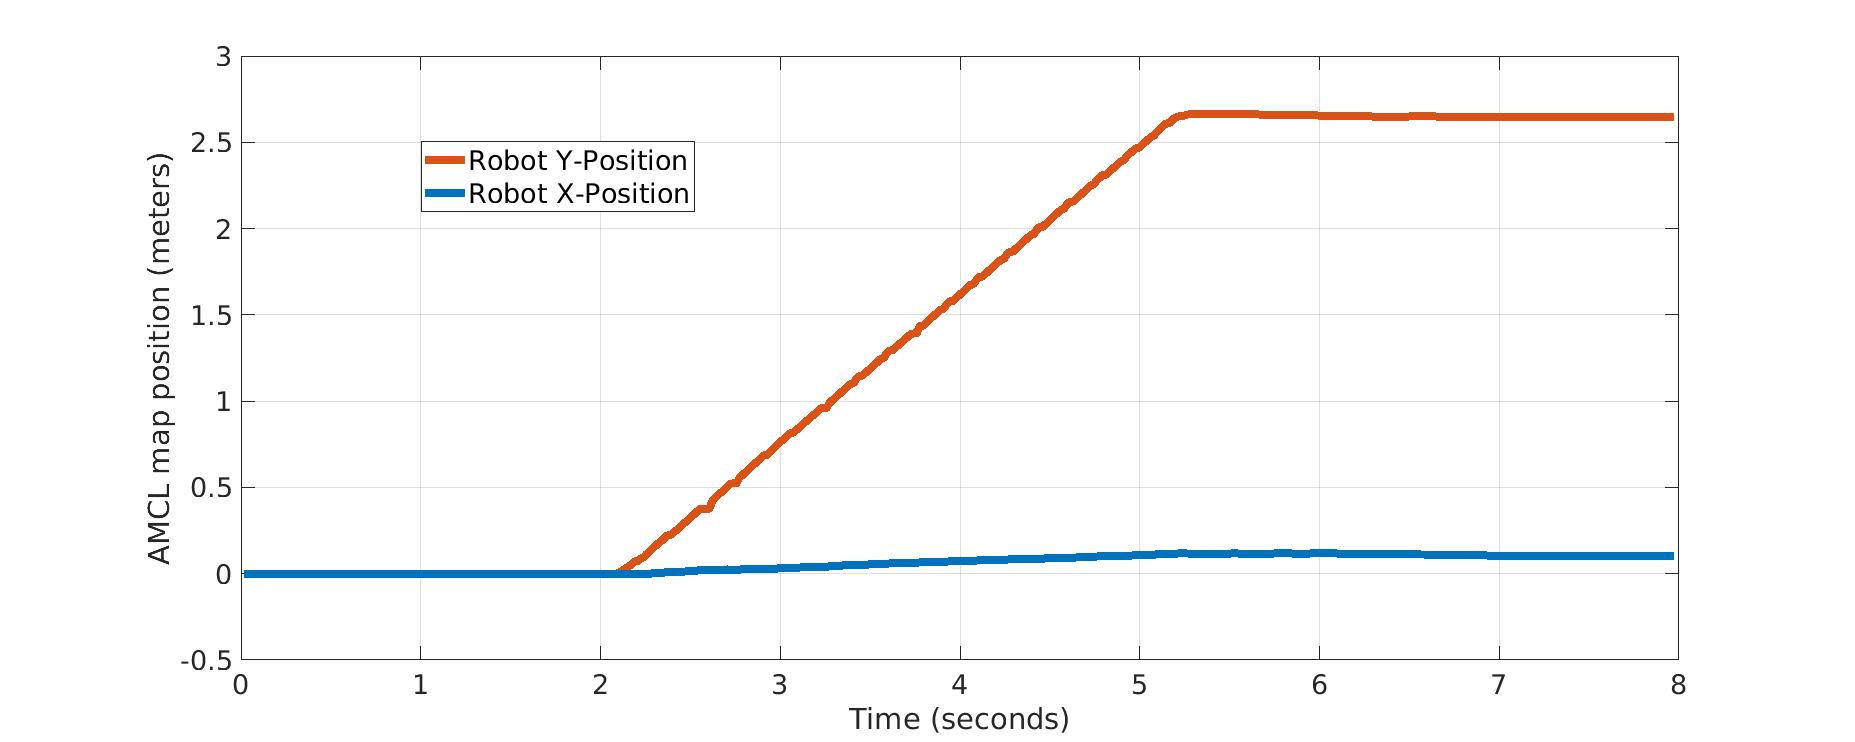
\includegraphics[width=12cm]{images/03-foundation/amcl14y}
	\caption{AMCL map position - 1.4m/s y-velocity set-point (slipping / no velocity smoothing).} 
	\label{amcl14y}
\end{figure}

\begin{figure}[H]
	\centering
	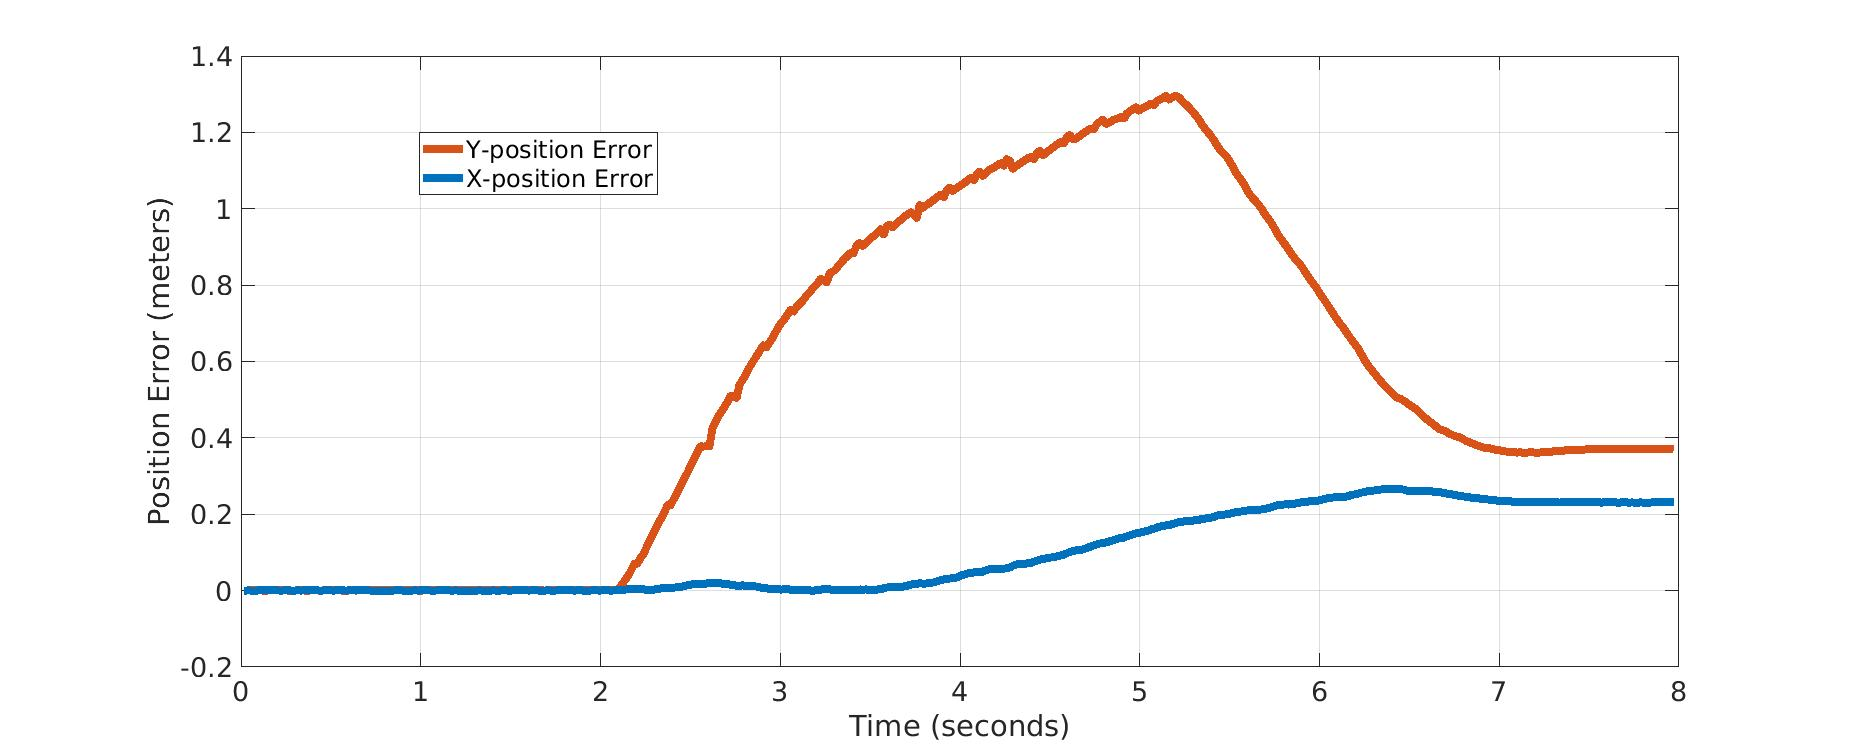
\includegraphics[width=12cm]{images/03-foundation/poserror14y}
	\caption{Position error - 1.4m/s y-velocity set-point (slipping / no velocity smoothing)} 
	\label{poserror14y}
\end{figure}

\begin{figure}[H]
	\centering
	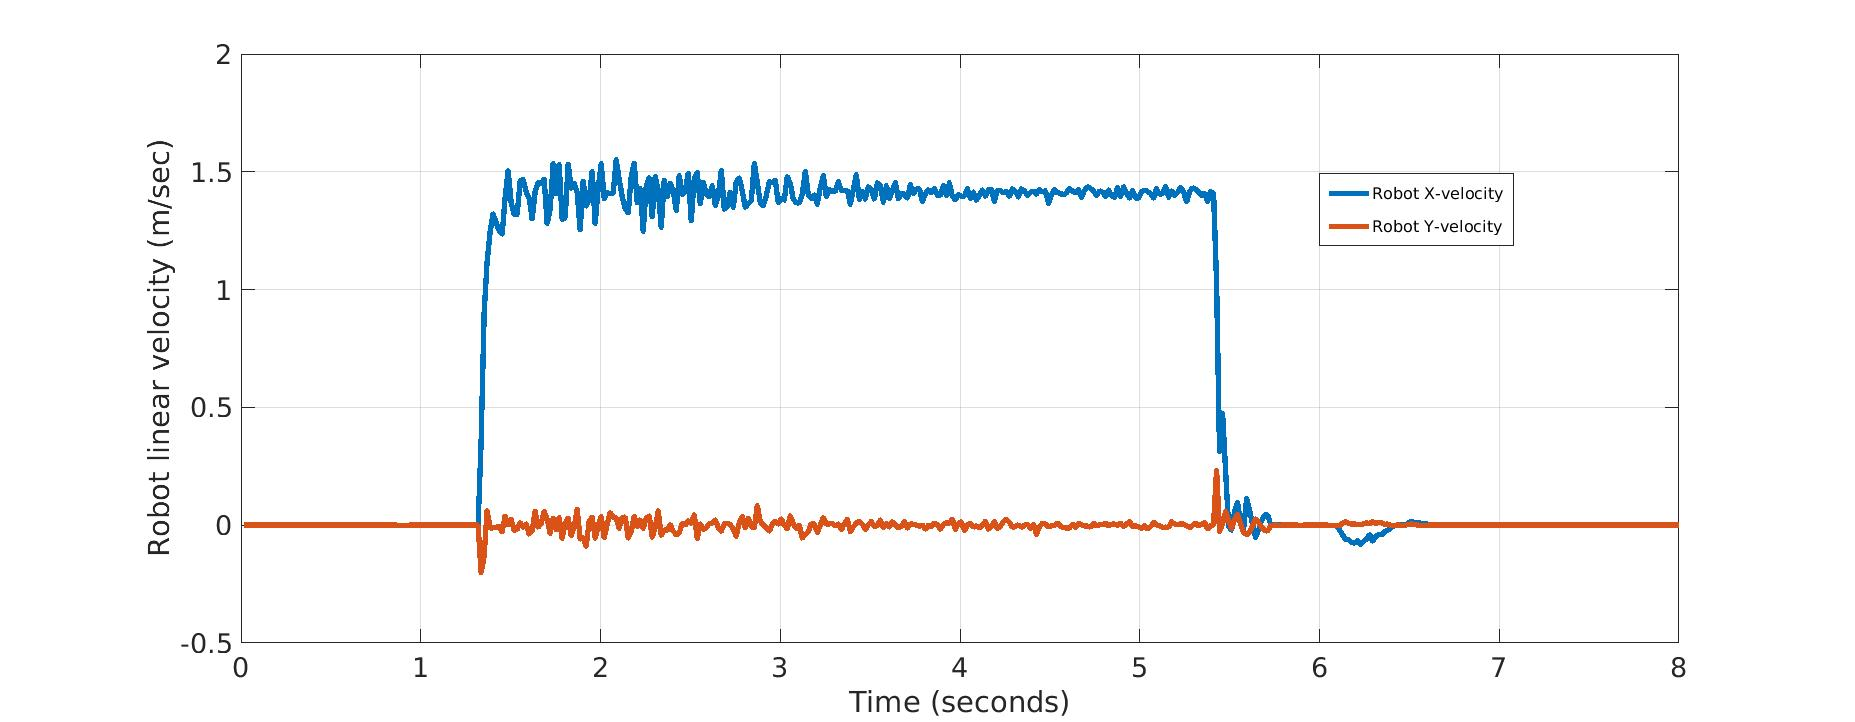
\includegraphics[width=12cm]{images/03-foundation/vel14}
	\caption{Robot measured linear velocity - 1.4m/s x-velocity set-point (slipping / no velocity smoothing)} 
	\label{vel14}
\end{figure}

\begin{figure}[H]
	\centering
	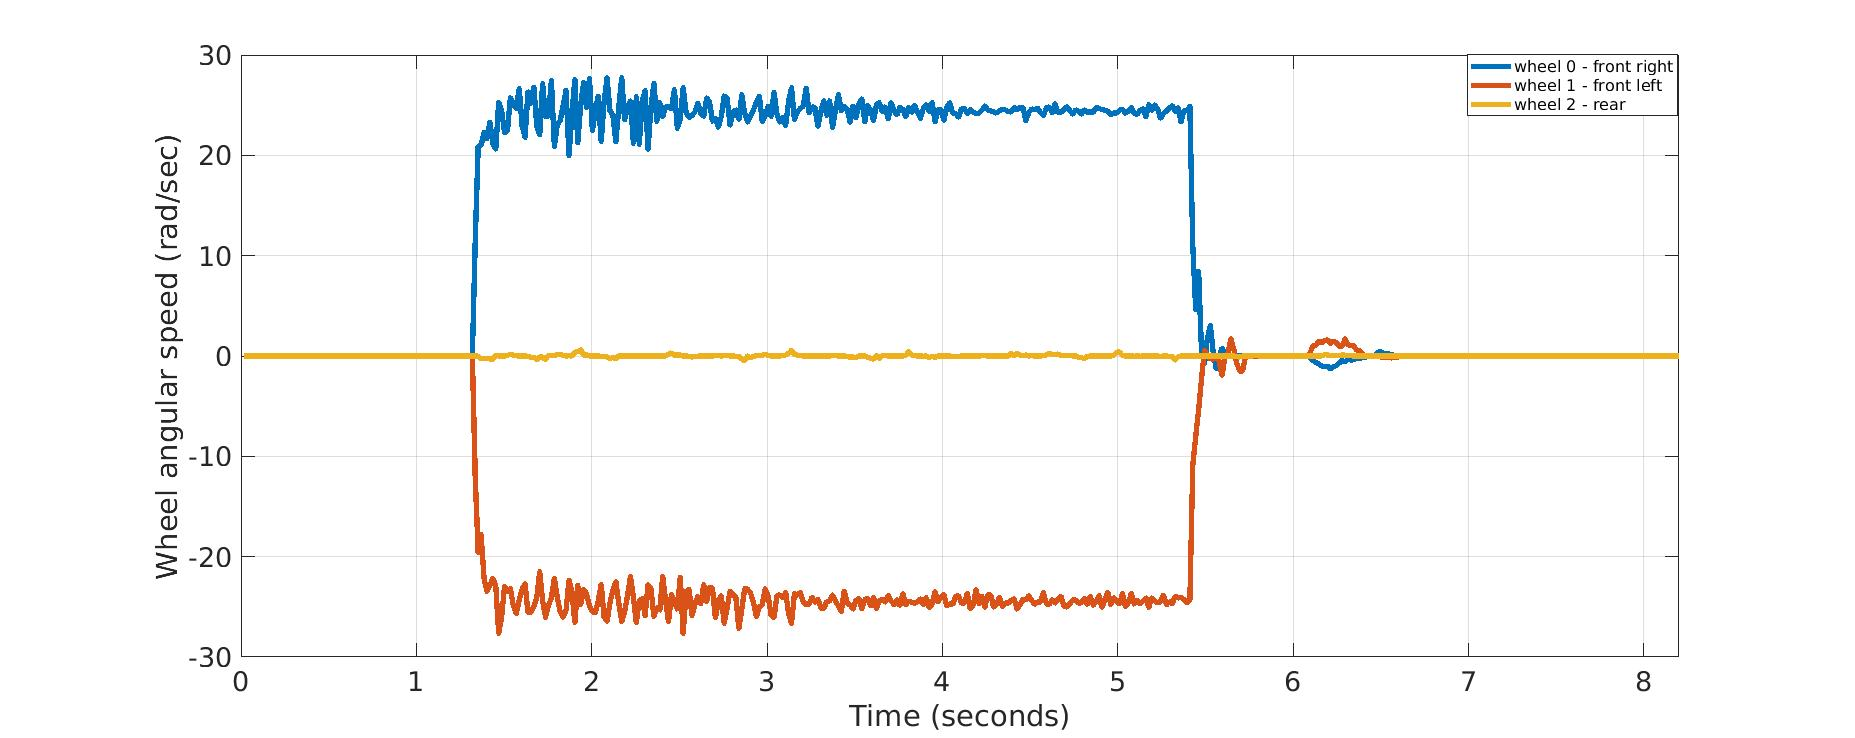
\includegraphics[width=12cm]{images/03-foundation/wheel14}
	\caption{wheels measured angular velocity - 1.4m/s x-velocity set-point (slipping / no velocity smoothing)} 
	\label{wheel14}
\end{figure}

\section{Fuzzy Rules} 
\subsection{Repulsive behavior if obstacles are encountered}

\begin{enumerate}
    \small
	\item \textbf{IF} $\left[\left( \text{min\_front\_left} == \textsf{close}\right) \textbf{ OR } \left(\text{min\_front\_right} == \textsf{close}\right)\right]$\\ 
	\textbf{THEN} $\Rightarrow\left[\left( V_x = \textsf{stop} \right) \textbf{AND} \left(V_y = -0.5\right)\right]$
	
	\item \textbf{IF} $ \left[\left( \text{min\_front\_left} == \textsf{far}\right) \textbf{ AND} \left(\text{min\_front\_right} == \textsf{far}\right) \textbf{AND} \left(\text{near\_goal} == \textsf{false}\right)
	\right]$\\ 
	\textbf{THEN} $\Rightarrow\left[\left( V_x = \textsf{stop} \right) \textbf{AND} \left(V_y = -0.4\right)\right]$
	
	\item \textbf{IF} [($\text{min\_rear\_left}$ == $\textsf{close}$) \textbf{AND} ($\text{index\_rear\_left}$ == $\textsf{is\_rear\_left}$)\\
	\textbf{AND} (near\_goal == \textsf{false})]
	\textbf{THEN} $\Rightarrow$ [( $V_x$ = \textsf{0.4}) \textbf{AND} ($V_y$ = \textsf{0.5})]
	
	\item \textbf{IF} [($\text{min\_rear\_left}$ == $\textsf{close}$) \textbf{AND} ($\text{index\_rear\_left}$ == $\textsf{is\_left}$)\\
	\textbf{AND} (near\_goal == \textsf{false})]		\textbf{THEN} $\Rightarrow$ [( $V_x$ = \textsf{0.5}) \textbf{AND} ($V_y$ = \textsf{0.4})]

	\item \textbf{IF} [($\text{min\_rear\_left}$ == $\textsf{far}$) \textbf{AND} ($\text{index\_rear\_left}$ == $\textsf{is\_rear\_left}$)\\
	\textbf{AND} (near\_goal == \textsf{false})]
	\textbf{THEN} $\Rightarrow$ [( $V_x$ = \textsf{0.3}) \textbf{AND} ($V_y$ = \textsf{0.4})]

	\item \textbf{IF} [($\text{min\_rear\_left}$ == $\textsf{far}$) \textbf{AND} ($\text{index\_rear\_left}$ == $\textsf{is\_left}$)\\
	\textbf{AND} (near\_goal == \textsf{false})]
	\textbf{THEN} $\Rightarrow$ [( $V_x$ = \textsf{0.4}) \textbf{AND} ($V_y$ = \textsf{0.3})]

	\item \textbf{IF} [($\text{min\_rear\_right}$ == $\textsf{close}$) \textbf{AND} ($\text{index\_rear\_right}$ == $\textsf{is\_rear\_right}$)\\
	\textbf{AND} (near\_goal == \textsf{false})]
	\textbf{THEN} $\Rightarrow$ [( $V_x$ = \textsf{-0.4}) \textbf{AND} ($V_y$ = \textsf{0.5})]	
	
	\item \textbf{IF} [($\text{min\_rear\_right}$ == $\textsf{close}$) \textbf{AND} ($\text{index\_rear\_right}$ == $\textsf{is\_right}$)\\
	\textbf{AND} (near\_goal == \textsf{false})]
	\textbf{THEN} $\Rightarrow$ [( $V_x$ = \textsf{-0.5}) \textbf{AND} ($V_y$ = \textsf{0.4})]
	
	\item \textbf{IF} [($\text{min\_rear\_right}$ == $\textsf{far}$) \textbf{AND} ($\text{index\_rear\_right}$ == $\textsf{is\_rear\_right}$)\\
	\textbf{AND} (near\_goal == \textsf{false})]
	\textbf{THEN} $\Rightarrow$ [( $V_x$ = \textsf{-0.3}) \textbf{AND} ($V_y$ = \textsf{0.4})]
	
	\item \textbf{IF} [($\text{min\_rear\_right}$ == $\textsf{far}$) \textbf{AND} ($\text{index\_rear\_right}$ == $\textsf{is\_right}$)\\
	\textbf{AND} (near\_goal == \textsf{false})]
	\textbf{THEN} $\Rightarrow$ [( $V_x$ = \textsf{-0.4}) \textbf{AND} ($V_y$ = \textsf{0.3})]
	
	\item \textbf{IF} [($\text{min\_left}$ == $\textsf{close}$) \textbf{AND} ($\text{index\_left}$ == $\textsf{is\_left}$)\\
	\textbf{AND} (near\_goal == \textsf{false})]
	\textbf{THEN} $\Rightarrow$ [( $V_x$ = \textsf{0.5}) \textbf{AND} ($V_y$ = \textsf{stop})]
	
	\item \textbf{IF} [($\text{min\_left}$ == $\textsf{close}$) \textbf{AND} ($\text{index\_left}$ == $\textsf{is\_rear\_left}$)\\
	\textbf{AND} (near\_goal == \textsf{false})]
	\textbf{THEN} $\Rightarrow$ [( $V_x$ = \textsf{0.5}) \textbf{AND} ($V_y$ = \textsf{0.2})]
	
	\item \textbf{IF} [($\text{min\_left}$ == $\textsf{close}$) \textbf{AND} ($\text{index\_left}$ == $\textsf{is\_front\_left}$)\\
	\textbf{AND} (near\_goal == \textsf{false})]
	\textbf{THEN} $\Rightarrow$ [( $V_x$ = \textsf{0.5}) \textbf{AND} ($V_y$ = \textsf{-0.2})]
	
	\item \textbf{IF} [($\text{min\_left}$ == $\textsf{far}$) \textbf{AND} ($\text{index\_left}$ == $\textsf{is\_left}$)\\
	\textbf{AND} (near\_goal == \textsf{false})]
	\textbf{THEN} $\Rightarrow$ [( $V_x$ = \textsf{0.4}) \textbf{AND} ($V_y$ = \textsf{stop})]
	
	\item \textbf{IF} [($\text{min\_left}$ == $\textsf{far}$) \textbf{AND} ($\text{index\_left}$ == $\textsf{is\_rear\_left}$)\\
	\textbf{AND} (near\_goal == \textsf{false})]
	\textbf{THEN} $\Rightarrow$ [( $V_x$ = \textsf{0.4}) \textbf{AND} ($V_y$ = \textsf{0.1})]
	
	\item \textbf{IF} [($\text{min\_left}$ == $\textsf{far}$) \textbf{AND} ($\text{index\_left}$ == $\textsf{is\_rear\_left}$)\\
	\textbf{AND} (near\_goal == \textsf{false})]
	\textbf{THEN} $\Rightarrow$ [( $V_x$ = \textsf{0.4}) \textbf{AND} ($V_y$ = \textsf{0.1})]
	
	\item \textbf{IF} [($\text{min\_right}$ == $\textsf{close}$) \textbf{AND} ($\text{index\_right}$ == $\textsf{is\_right}$)\\
	\textbf{AND} (near\_goal == \textsf{false})]
	\textbf{THEN} $\Rightarrow$ [( $V_x$ = \textsf{-0.5}) \textbf{AND} ($V_y$ = \textsf{stop})]
	
	\item \textbf{IF} [($\text{min\_right}$ == $\textsf{close}$) \textbf{AND} ($\text{index\_right}$ == $\textsf{is\_rear\_right}$)\\
	\textbf{AND} (near\_goal == \textsf{false})]
	\textbf{THEN} $\Rightarrow$ [( $V_x$ = \textsf{-0.5}) \textbf{AND} ($V_y$ = \textsf{0.2})]
	
	\item \textbf{IF} [($\text{min\_right}$ == $\textsf{close}$) \textbf{AND} ($\text{index\_right}$ == $\textsf{is\_front\_right}$)\\
	\textbf{AND} (near\_goal == \textsf{false})]
	\textbf{THEN} $\Rightarrow$ [( $V_x$ = \textsf{-0.5}) \textbf{AND} ($V_y$ = \textsf{-0.2})]
	
	\item \textbf{IF} [($\text{min\_right}$ == $\textsf{far}$) \textbf{AND} ($\text{index\_right}$ == $\textsf{is\_right}$)\\
	\textbf{AND} (near\_goal == \textsf{false})]
	\textbf{THEN} $\Rightarrow$ [( $V_x$ = \textsf{-0.4}) \textbf{AND} ($V_y$ = \textsf{stop})]
	
	\item \textbf{IF} [($\text{min\_right}$ == $\textsf{far}$) \textbf{AND} ($\text{index\_right}$ == $\textsf{is\_rear\_right}$)\\
	\textbf{AND} (near\_goal == \textsf{false})]
	\textbf{THEN} $\Rightarrow$ [( $V_x$ = \textsf{-0.4}) \textbf{AND} ($V_y$ = \textsf{0.1})]
	
	\item \textbf{IF} [($\text{min\_right}$ == $\textsf{far}$) \textbf{AND} ($\text{index\_right}$ == $\textsf{is\_front\_right}$)\\
	\textbf{AND} (near\_goal == \textsf{false})]
	\textbf{THEN} $\Rightarrow$ [( $V_x$ = \textsf{-0.4}) \textbf{AND} ($V_y$ = \textsf{-0.1})]
	
	\item \textbf{IF} [($\text{min\_rear\_left}$ == $\textsf{dontcare}$) 
	\textbf{AND} ($\text{min\_left}$ == $\textsf{dontcare}$)\\
	\textbf{AND} ($\text{min\_front\_left}$ == $\textsf{far}$)
	\textbf{AND} ($\text{min\_front\_right}$ == $\textsf{dontcare}$)\\
	\textbf{AND} ($\text{min\_right}$ == $\textsf{dontcare}$) 
	\textbf{AND} ($\text{min\_rear\_right}$ == $\textsf{dontcare}$) \\
	\textbf{AND} ($\text{index\_front\_left}$ == $\textsf{is\_front\_left}$)
	\textbf{AND} (near\_goal == \textsf{false})]\\
	\textbf{THEN} $\Rightarrow$ [( $V_x$ = \textsf{stop}) \textbf{AND} ($V_y$ = \textsf{-0.3})]

	\item \textbf{IF} [($\text{min\_rear\_left}$ == $\textsf{dontcare}$) 
	\textbf{AND} ($\text{min\_left}$ == $\textsf{dontcare}$)\\
	\textbf{AND} ($\text{min\_front\_left}$ == $\textsf{far}$)
	\textbf{AND} ($\text{min\_front\_right}$ == $\textsf{dontcare}$)\\
	\textbf{AND} ($\text{min\_right}$ == $\textsf{dontcare}$) 
	\textbf{AND} ($\text{min\_rear\_right}$ == $\textsf{dontcare}$) \\
	\textbf{AND} ($\text{index\_front\_left}$ == $\textsf{is\_left}$)
	\textbf{AND} (near\_goal == \textsf{false})]\\
	\textbf{THEN} $\Rightarrow$ [( $V_x$ = \textsf{0.3}) \textbf{AND} ($V_y$ = \textsf{-0.1})]
	
	\item \textbf{IF} [($\text{min\_rear\_left}$ == $\textsf{dontcare}$) 
	\textbf{AND} ($\text{min\_left}$ == $\textsf{dontcare}$)\\
	\textbf{AND} ($\text{min\_front\_left}$ == $\textsf{far}$)
	\textbf{AND} ($\text{min\_front\_right}$ == $\textsf{dontcare}$)\\
	\textbf{AND} ($\text{min\_right}$ == $\textsf{dontcare}$) 
	\textbf{AND} ($\text{min\_rear\_right}$ == $\textsf{dontcare}$) \\
	\textbf{AND} ($\text{index\_front\_left}$ == $\textsf{is\_front\_right}$)
	\textbf{AND} (near\_goal == \textsf{false})]\\
	\textbf{THEN} $\Rightarrow$ [( $V_x$ = \textsf{-0.3}) \textbf{AND} ($V_y$ = \textsf{-0.1})]
	
	\item \textbf{IF} [($\text{min\_rear\_left}$ == $\textsf{dontcare}$) 
	\textbf{AND} ($\text{min\_left}$ == $\textsf{dontcare}$)\\
	\textbf{AND} ($\text{min\_front\_left}$ == $\textsf{close}$)
	\textbf{AND} ($\text{min\_front\_right}$ == $\textsf{dontcare}$)\\
	\textbf{AND} ($\text{min\_right}$ == $\textsf{dontcare}$) 
	\textbf{AND} ($\text{min\_rear\_right}$ == $\textsf{dontcare}$) \\
	\textbf{AND} ($\text{index\_front\_left}$ == $\textsf{is\_front\_left}$)
	\textbf{AND} (near\_goal == \textsf{false})]\\
	\textbf{THEN} $\Rightarrow$ [( $V_x$ = \textsf{stop}) \textbf{AND} ($V_y$ = \textsf{-0.3})]
	
	\item \textbf{IF} [($\text{min\_rear\_left}$ == $\textsf{dontcare}$) 
	\textbf{AND} ($\text{min\_left}$ == $\textsf{dontcare}$)\\
	\textbf{AND} ($\text{min\_front\_left}$ == $\textsf{close}$)
	\textbf{AND} ($\text{min\_front\_right}$ == $\textsf{dontcare}$)\\
	\textbf{AND} ($\text{min\_right}$ == $\textsf{dontcare}$) 
	\textbf{AND} ($\text{min\_rear\_right}$ == $\textsf{dontcare}$) \\
	\textbf{AND} ($\text{index\_front\_left}$ == $\textsf{is\_left}$)
	\textbf{AND} (near\_goal == \textsf{false})]\\
	\textbf{THEN} $\Rightarrow$ [( $V_x$ = \textsf{0.3}) \textbf{AND} ($V_y$ = \textsf{-0.2})]
	
	\item \textbf{IF} [($\text{min\_rear\_left}$ == $\textsf{dontcare}$) 
	\textbf{AND} ($\text{min\_left}$ == $\textsf{dontcare}$)\\
	\textbf{AND} ($\text{min\_front\_left}$ == $\textsf{close}$)
	\textbf{AND} ($\text{min\_front\_right}$ == $\textsf{dontcare}$)\\
	\textbf{AND} ($\text{min\_right}$ == $\textsf{dontcare}$) 
	\textbf{AND} ($\text{min\_rear\_right}$ == $\textsf{dontcare}$) \\
	\textbf{AND} ($\text{index\_front\_left}$ == $\textsf{is\_front\_right}$)
	\textbf{AND} (near\_goal == \textsf{false})]\\
	\textbf{THEN} $\Rightarrow$ [( $V_x$ = \textsf{-0.3}) \textbf{AND} ($V_y$ = \textsf{-0.2})]
	
	\item \textbf{IF} [($\text{min\_rear\_left}$ == $\textsf{dontcare}$) 
	\textbf{AND} ($\text{min\_left}$ == $\textsf{dontcare}$)\\
	\textbf{AND} ($\text{min\_front\_left}$ == $\textsf{dontcare}$)
	\textbf{AND} ($\text{min\_front\_right}$ == $\textsf{far}$)\\
	\textbf{AND} ($\text{min\_right}$ == $\textsf{dontcare}$) 
	\textbf{AND} ($\text{min\_rear\_right}$ == $\textsf{dontcare}$) \\
	\textbf{AND} ($\text{index\_front\_right}$ == $\textsf{is\_front\_right}$)
	\textbf{AND} (near\_goal == \textsf{false})]\\
	\textbf{THEN} $\Rightarrow$ [( $V_x$ = \textsf{stop}) \textbf{AND} ($V_y$ = \textsf{-0.3})]

	\item \textbf{IF} [($\text{min\_rear\_left}$ == $\textsf{dontcare}$) 
	\textbf{AND} ($\text{min\_left}$ == $\textsf{dontcare}$)\\
	\textbf{AND} ($\text{min\_front\_left}$ == $\textsf{dontcare}$)
	\textbf{AND} ($\text{min\_front\_right}$ == $\textsf{far}$)\\
	\textbf{AND} ($\text{min\_right}$ == $\textsf{dontcare}$) 
	\textbf{AND} ($\text{min\_rear\_right}$ == $\textsf{dontcare}$) \\
	\textbf{AND} ($\text{index\_front\_right}$ == $\textsf{is\_right}$)
	\textbf{AND} (near\_goal == \textsf{false})]\\
	\textbf{THEN} $\Rightarrow$ [( $V_x$ = \textsf{-0.3}) \textbf{AND} ($V_y$ = \textsf{-0.1})]
	
	\item \textbf{IF} [($\text{min\_rear\_left}$ == $\textsf{dontcare}$) 
	\textbf{AND} ($\text{min\_left}$ == $\textsf{dontcare}$)\\
	\textbf{AND} ($\text{min\_front\_left}$ == $\textsf{dontcare}$)
	\textbf{AND} ($\text{min\_front\_right}$ == $\textsf{far}$)\\
	\textbf{AND} ($\text{min\_right}$ == $\textsf{dontcare}$) 
	\textbf{AND} ($\text{min\_rear\_right}$ == $\textsf{dontcare}$) \\
	\textbf{AND} ($\text{index\_front\_right}$ == $\textsf{is\_front\_right}$)
	\textbf{AND} (near\_goal == \textsf{false})]\\
	\textbf{THEN} $\Rightarrow$ [( $V_x$ = \textsf{0.3}) \textbf{AND} ($V_y$ = \textsf{-0.1})]	
	
	\item \textbf{IF} [($\text{min\_rear\_left}$ == $\textsf{dontcare}$) 
	\textbf{AND} ($\text{min\_left}$ == $\textsf{dontcare}$)\\
	\textbf{AND} ($\text{min\_front\_left}$ == $\textsf{dontcare}$)
	\textbf{AND} ($\text{min\_front\_right}$ == $\textsf{close}$)\\
	\textbf{AND} ($\text{min\_right}$ == $\textsf{dontcare}$) 
	\textbf{AND} ($\text{min\_rear\_right}$ == $\textsf{dontcare}$) \\
	\textbf{AND} ($\text{index\_front\_right}$ == $\textsf{is\_front\_right}$)
	\textbf{AND} (near\_goal == \textsf{false})]\\
	\textbf{THEN} $\Rightarrow$ [( $V_x$ = \textsf{stop}) \textbf{AND} ($V_y$ = \textsf{-0.3})]
	
	\item \textbf{IF} [($\text{min\_rear\_left}$ == $\textsf{dontcare}$) 
	\textbf{AND} ($\text{min\_left}$ == $\textsf{dontcare}$)\\
	\textbf{AND} ($\text{min\_front\_left}$ == $\textsf{dontcare}$)
	\textbf{AND} ($\text{min\_front\_right}$ == $\textsf{close}$)\\
	\textbf{AND} ($\text{min\_right}$ == $\textsf{dontcare}$) 
	\textbf{AND} ($\text{min\_rear\_right}$ == $\textsf{dontcare}$) \\
	\textbf{AND} ($\text{index\_front\_right}$ == $\textsf{is\_right}$)
	\textbf{AND} (near\_goal == \textsf{false})]\\
	\textbf{THEN} $\Rightarrow$ [( $V_x$ = \textsf{-0.3}) \textbf{AND} ($V_y$ = \textsf{-0.2})]
	
	\item \textbf{IF} [($\text{min\_rear\_left}$ == $\textsf{dontcare}$) 
	\textbf{AND} ($\text{min\_left}$ == $\textsf{dontcare}$)\\
	\textbf{AND} ($\text{min\_front\_left}$ == $\textsf{dontcare}$)
	\textbf{AND} ($\text{min\_front\_right}$ == $\textsf{close}$)\\
	\textbf{AND} ($\text{min\_right}$ == $\textsf{dontcare}$) 
	\textbf{AND} ($\text{min\_rear\_right}$ == $\textsf{dontcare}$) \\
	\textbf{AND} ($\text{index\_front\_right}$ == $\textsf{is\_front\_right}$)
	\textbf{AND} (near\_goal == \textsf{false})]\\
	\textbf{THEN} $\Rightarrow$ [( $V_x$ = \textsf{0.3}) \textbf{AND} ($V_y$ = \textsf{-0.2})]
\end{enumerate}

\subsection{Attractive behavior if near towers}

\begin{enumerate}
    \small
	\item \textbf{IF} [($\text{min\_rear\_left}$ == $\textsf{dontcare}$) 
	\textbf{AND} ($\text{min\_left}$ == $\textsf{dontcare}$)\\
	\textbf{AND} ($\text{min\_front\_left}$ == $\textsf{dontcare}$)
	\textbf{AND} ($\text{min\_front\_right}$ == $\textsf{dontcare}$)\\
	\textbf{AND} ($\text{min\_right}$ == $\textsf{dontcare}$) 
	\textbf{AND} ($\text{min\_rear\_right}$ == $\textsf{dontcare}$) \\
	\textbf{AND} (near\_goal == \textsf{true})]
	\textbf{THEN} $\Rightarrow$ [( $V_x$ = \textsf{stop}) \textbf{AND} ($V_y$ = \textsf{-0.5})]
	
	\item \textbf{IF} [($\text{min\_rear\_left}$ == $\textsf{dontcare}$) 
	\textbf{AND} ($\text{min\_left}$ == $\textsf{dontcare}$)\\
	\textbf{AND} ($\text{min\_front\_left}$ == $\textsf{dontcare}$)
	\textbf{AND} ($\text{min\_front\_right}$ == $\textsf{dontcare}$)\\
	\textbf{AND} ($\text{min\_right}$ == $\textsf{dontcare}$) 
	\textbf{AND} ($\text{min\_rear\_right}$ == $\textbf{not } \textsf{dontcare}$)\\
	\textbf{AND} (near\_goal == \textsf{true})]
	\textbf{THEN} $\Rightarrow$ [( $V_x$ = \textsf{0.4}) \textbf{AND} ($V_y$ = \textsf{-0.4})]
	
	\item \textbf{IF} [($\textbf{not }\text{min\_rear\_left}$ == $\textsf{\textbf{not }dontcare}$) 
	\textbf{AND} ($\text{min\_left}$ == $\textsf{dontcare}$)\\
	\textbf{AND} ($\text{min\_front\_left}$ == $\textsf{dontcare}$)
	\textbf{AND} ($\text{min\_front\_right}$ == $\textsf{dontcare}$)\\
	\textbf{AND} ($\text{min\_right}$ == $\textsf{dontcare}$) 
	\textbf{AND} ($\text{min\_rear\_right}$ == $\textsf{dontcare}$)\\
	\textbf{AND} (near\_goal == \textsf{true})]
	\textbf{THEN} $\Rightarrow$ [( $V_x$ = \textsf{-0.4}) \textbf{AND} ($V_y$ = \textsf{0.4})]
	
	\item \textbf{IF} [($\text{min\_rear\_left}$ == $\textsf{dontcare}$) 
	\textbf{AND} ($\textbf{not }\text{min\_left}$ == $\textsf{dontcare}$)\\
	\textbf{AND} ($\text{min\_front\_left}$ == $\textsf{dontcare}$)
	\textbf{AND} ($\text{min\_front\_right}$ == $\textsf{dontcare}$)\\
	\textbf{AND} ($\text{min\_right}$ == $\textsf{dontcare}$) 
	\textbf{AND} ($\text{min\_rear\_right}$ == $\textsf{dontcare}$)\\
	\textbf{AND} (near\_goal == \textsf{true})]
	\textbf{THEN} $\Rightarrow$ [( $V_x$ = \textsf{-0.4}) \textbf{AND} ($V_y$ = \textsf{-0.1})]
	
	\item \textbf{IF} [($\text{min\_rear\_left}$ == $\textsf{dontcare}$) 
	\textbf{AND} ($\text{min\_left}$ == $\textsf{dontcare}$)\\
	\textbf{AND} ($\text{min\_front\_left}$ == $\textsf{dontcare}$)
	\textbf{AND} ($\text{min\_front\_right}$ == $\textsf{dontcare}$)\\
	\textbf{AND} ($\textbf{not }\text{min\_right}$ == $\textsf{dontcare}$) 
	\textbf{AND} ($\text{min\_rear\_right}$ == $\textsf{dontcare}$)\\
	\textbf{AND} (near\_goal == \textsf{true})]
	\textbf{THEN} $\Rightarrow$ [( $V_x$ = \textsf{0.4}) \textbf{AND} ($V_y$ = \textsf{-0.1})]
	
	\item \textbf{IF} [($\textbf{not }\text{min\_rear\_left}$ == $\textsf{dontcare}$) 
	\textbf{AND} ($\text{min\_left}$ == $\textsf{dontcare}$)\\
	\textbf{AND} ($\text{min\_front\_left}$ == $\textsf{\textbf{not }dontcare}$)
	\textbf{AND} ($\text{min\_front\_right}$ == $\textsf{dontcare}$)\\
	\textbf{AND} ($\text{min\_right}$ == $\textsf{dontcare}$) 
	\textbf{AND} ($\text{min\_rear\_right}$ == $\textsf{\textbf{not }dontcare}$)\\
	\textbf{AND} (near\_goal == \textsf{true})]
	\textbf{THEN} $\Rightarrow$ [( $V_x$ = \textsf{stop}) \textbf{AND} ($V_y$ = \textsf{-0.4})]
	
	\item \textbf{IF} [($\text{min\_rear\_left}$ == $\textsf{dontcare}$) 
	\textbf{AND} ($\text{min\_left}$ == $\textsf{dontcare}$)\\
	\textbf{AND} ($\text{min\_front\_left}$ == $\textsf{dontcare}$)
	\textbf{AND} ($\text{min\_front\_right}$ == $\textsf{dontcare}$)\\
	\textbf{AND} ($\text{min\_right}$ == $\textsf{\textbf{not }dontcare}$) 
	\textbf{AND} ($\text{min\_rear\_right}$ == $\textsf{\textbf{not }dontcare}$)\\
	\textbf{AND} (near\_goal == \textsf{true})]
	\textbf{THEN} $\Rightarrow$ [( $V_x$ = \textsf{0.4}) \textbf{AND} ($V_y$ = \textsf{-0.3})]
	
	\item \textbf{IF} [($\textbf{not }\text{min\_rear\_left}$ == $\textsf{dontcare}$) 
	\textbf{AND} ($\textbf{not }\text{min\_left}$ == $\textsf{dontcare}$)\\
	\textbf{AND} ($\text{min\_front\_left}$ == $\textsf{dontcare}$)
	\textbf{AND} ($\text{min\_front\_right}$ == $\textsf{dontcare}$)\\
	\textbf{AND} ($\text{min\_right}$ == $\textsf{\textbf{not }dontcare}$) 
	\textbf{AND} ($\text{min\_rear\_right}$ == $\textsf{dontcare}$)\\
	\textbf{AND} (near\_goal == \textsf{true})]
	\textbf{THEN} $\Rightarrow$ [( $V_x$ = \textsf{-0.4}) \textbf{AND} ($V_y$ = \textsf{-0.3})]
\end{enumerate}
